
\documentclass[12pt]{article}
\usepackage[utf8]{inputenc}
\usepackage{subfiles}
\usepackage{lipsum}
\usepackage[linesnumbered,algoruled,boxed]{algorithm2e}
\usepackage{hyperref}
\usepackage{listings}
\usepackage{color}
\usepackage{tikz}
\usepackage[english]{babel}
\usepackage{natbib}
\usepackage{url}
\usepackage{graphicx}
\graphicspath{{images/}}
\usepackage{parskip}
\usepackage{fancyhdr}
\usepackage{vmargin}

\usepackage{array}
\usepackage{subcaption}
\usepackage{xparse}


\definecolor{codegreen}{rgb}{0,0.6,0}
\definecolor{codegray}{rgb}{0.5,0.5,0.5}
\definecolor{codepurple}{rgb}{0.58,0,0.82}
\definecolor{backcolour}{rgb}{0.95,0.95,0.92}



\lstdefinestyle{mystyle}{
    backgroundcolor=\color{backcolour},   
    commentstyle=\color{codegreen},
    keywordstyle=\color{magenta},
    numberstyle=\tiny\color{codegray},
    stringstyle=\color{blue},
    basicstyle=\footnotesize,
    breakatwhitespace=false,         
    breaklines=true,                 
    captionpos=b,                    
    keepspaces=true,                 
    numbers=right,                    
    numbersep=5pt,                  
    showspaces=false,                
    showstringspaces=false,
    showtabs=false,                  
    tabsize=8
}

\lstset{style=mystyle}



\setmarginsrb{3 cm}{2.5 cm}{3 cm}{2.5 cm}{1 cm}{1.5 cm}{1 cm}{1.5 cm}


\title{DHCP Spoofing} 			
\author{1505118}								
\date{\today}									

\makeatletter
\let\thetitle\@title
\let\theauthor\@author
\let\thedate\@date
\makeatother

\pagestyle{fancy}
\fancyhf{}
\rhead{\theauthor}
\lhead{\thetitle}
\cfoot{\thepage}



\begin{document}

%%%%%%%%%%%%%%%%%%%%%%%%%%%%%%%%%%%%%%%%%%%%%%%%%%%%%%%%%%%%%%%%%%%%%%%%%%%%%%%%%%%%%%%%%

\begin{titlepage}
	\centering
    \vspace*{0.5 cm}
    
    %\includegraphics[scale = 0.75]{logo}\\[1.0 cm]	% University Logo
    \textsc{\LARGE Bangladesh University of Engineering \newline\newline and Technology}\\[2.0 cm]	% University Name
	\textsc{\Large Security Project}\\[0.5 cm]				% Course Code
	\rule{\linewidth}{0.2 mm} \\[0.4 cm]
	{ \huge \bfseries \thetitle}\\
	\rule{\linewidth}{0.2 mm} \\[1.5 cm]
	
		\begin{minipage}{0.4\textwidth}
		\begin{center} 
		\textsc{\Large \emph{Submitted By :} \\
					Afsara Benazir\\
					1505118}\\[0.5 cm]	
		\end{center}
		\end{minipage}~
		
		    
		
	

\end{titlepage}

%%%%%%%%%%%%%%%%%%%%%%%%%%%%%%%%%%%%%%%%%%%%%%%%%%%%%%%%%%%%%%%%%%%%%%%%%%%%%%%%%%%%%%%%%

%\maketitle
\tableofcontents

\section{Introduction}



\begin{sloppypar}
	
DHCP spoofing occurs when an attacker attempts to respond to DHCP requests and trying to list themselves (spoofs) as the default gateway or DNS server, hence, initiating a man in the middle attack. With that, it is possible that they can intercept traffic from users before forwarding to the real gateway or perform DoS by flooding the real DHCP server with request to choke IP address resources.

DHCP Starvation attack is a common network attack that targets network DHCP servers. Its primary objective is to flood the organization’s DHCP server with DHCP REQUEST messages using spoofed source MAC addresses. The DHCP server will respond to all requests, not knowing this is a DHCP Starvation attack, and assign available IP addresses until its DHCP pool is depleted.


After a DHCP starvation attack and setting up a rogue DHCP server, the attacker can start distributing IP addresses and other TCP/IP configuration settings to the network DHCP clients. TCP/IP configuration settings include Default Gateway and DNS Server IP addresses. Network attackers can now replace the original legitimate Default Gateway IP Address and DNS Server IP Address with their own IP Address.

Once the Default Gateway IP Address of the network devices are is changed, the network clients start sending the traffic destined to outside networks to the attacker's computer. The attacker can now capture sensitive user data and launch a man-in-the-middle attack. This is called as DHCP spoofing attack. Attacker can also set up a rogue DNS server and deviate the end user traffic to fake web sites and launch phishing attacks.

\section{How DHCP Works?}

\begin{sloppypar}
	
	A DHCP server is used to issue unique IP addresses and automatically configure other network information (the DNS domain name and the IP address of the default router, of the DNS server and of the NetBIOS name server).
	
	This configuration, is allocated to the device only for a given time: the lease time.
	
	
	Basically, mostly in homes and small networks, the DHCP Server is situated in the Router and in large organizational sectors, DHCP Server can be an individual computer also. A DHCP server provides this information to a DHCP client through the exchange of a series of messages, known as the DHCP conversation or the DHCP transaction.
	
	
	A typical DHCP exchange is as follows :
	\begin{enumerate}
		
		\item \texttt{\underline{DISCOVER:}} The client without IP address configured sends this query to obtain one from the DHCP server. As the client has no information whatsoever about the current network configuration, not even the address of the DHCPserver, the request is broadcasted on the local subnet. The client may already ask for a previously leased IP address.
		
		The server search on its side for a free address he can allocate to the client. This usually involves two mechanisms:
		The server maintains a local database of leased and available IP addresses.
		Once an address candidate has been selected, depending on the server implementation the server may take great care that the IP is indeed not already used by sending one or two ARP requests with relatively large waiting time for any potential answer.
		
		\item \texttt{\underline{OFFER:}} The server proposes the address to the client. For availability purposes DHCP allows several servers to send concurrent offers, the client choosing the “best” one. This message is usually sent as unicast to the client MAC address.
		
		\item \texttt{\underline{REQUEST:}} The client broadcasts the address it has chosen. This allows all DHCP servers involved in this exchange to be aware of the client’s decision.
		Clients wanting to renew an already acquired lease first attempt to directly jump to this step of the discussion by sending a unicast DHCP REQUEST message to the DHCP server which issued the lease.
		
		\item \texttt{\underline{ACKNOWLEDGEMENT:}} The server acknowledges the client decision and provides him complementary network configuration settings 
	\end{enumerate}
	
	
	\begin{figure}[h]
		\centering
		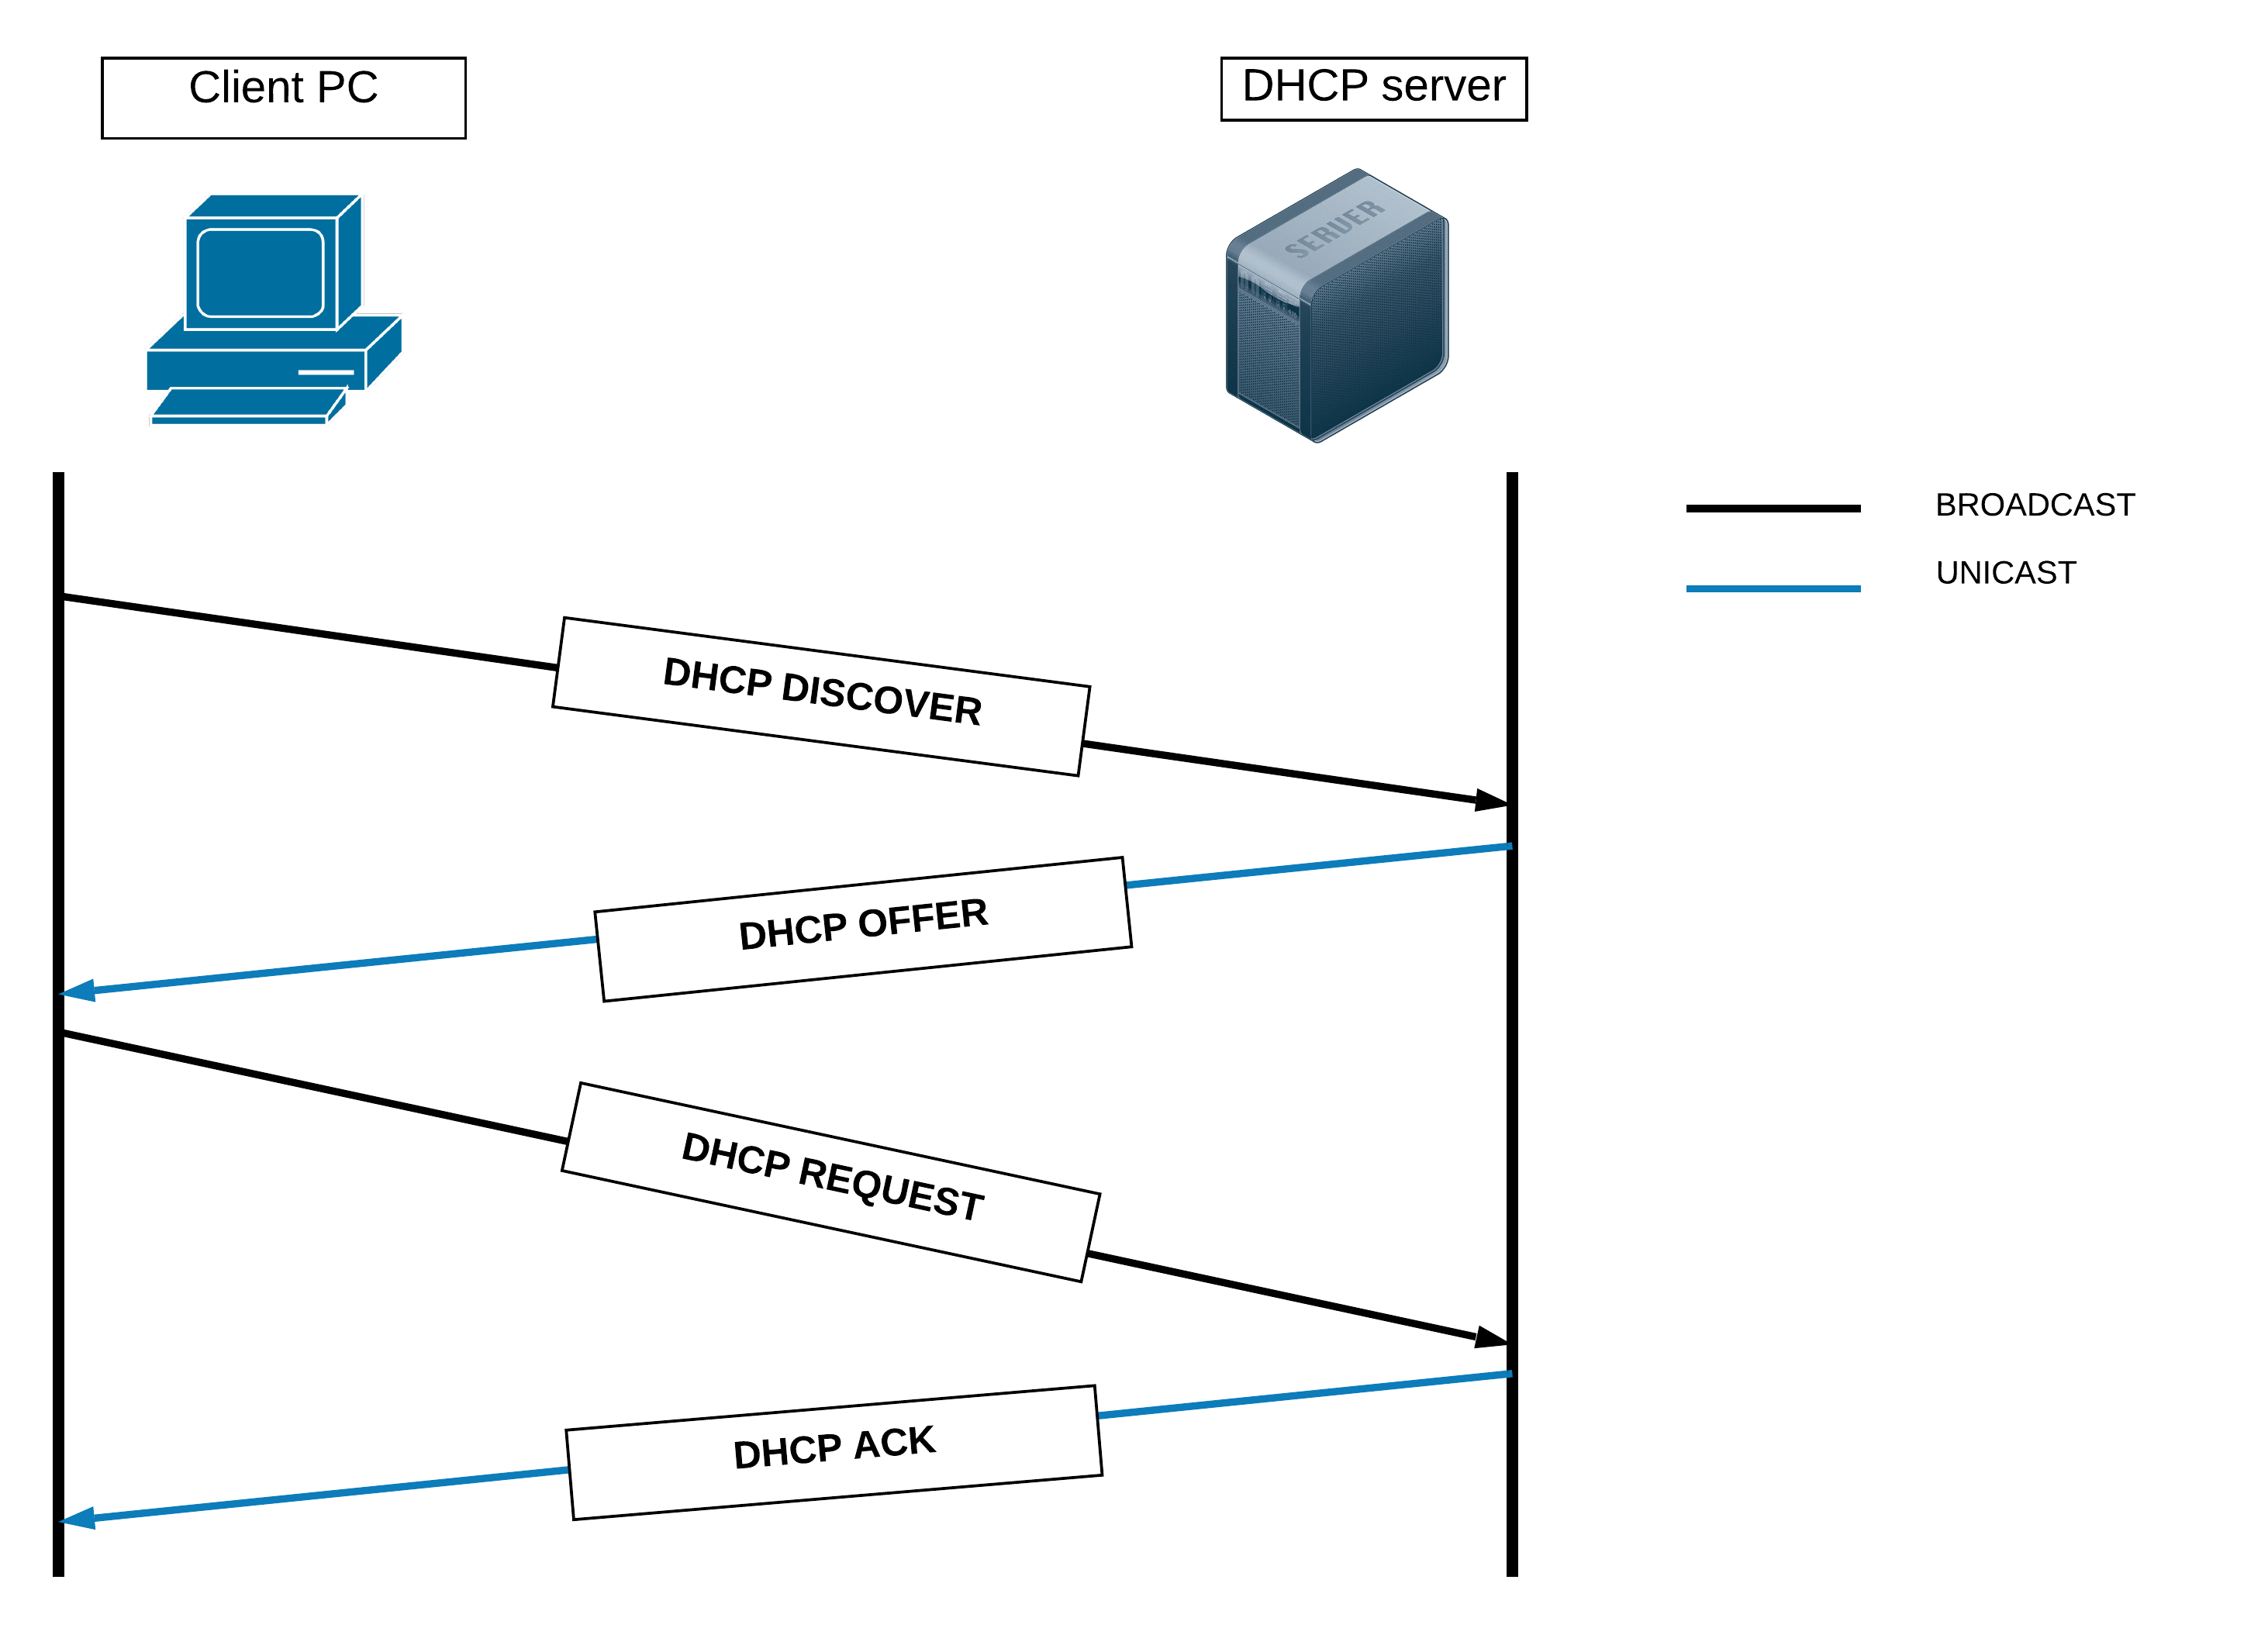
\includegraphics[width=12 cm,height=9 cm]{images/DHCP.png};
		\caption{Timing diagram of the original protocol}
	\end{figure}
	
\end{sloppypar}

\section{Definition of the attack with topology diagram}

\begin{sloppypar}
	
	In the context of information security, and especially network security, a spoofing attack is a situation in which a person or program successfully masquerades as another by falsifying data, to gain an illegitimate advantage.
	
	
	\textbf{DHCP spoofing occurs when an attacker attempts to respond to DHCP requests and trying to list themselves (spoofs) as the default gateway or DNS server, hence, initiating a man in the middle attack. With that, it is possible that they can intercept traffic from users before forwarding to the real gateway or perform DoS by flooding the real DHCP server with request to choke IP address resources.}
	
	
	
	\subsection{\texttt{\underline{Rogue DHCP Server : } }}
	
	
	
	DHCP Discover traffic are sent as broadcasts and are therefore observable to all devices on the LAN.  An attacker connected to the broadcast domain can opportunistically listen for these broadcasts and attempt to respond with an Offer before the real server.  This allows an attacker to feed endpoints malicious DHCP lease information that include changes such as an alternative default gateway or DNS server value in order to redirect traffic through the attacker’s endpoint to create a man-in-the-middle attack. At the very least it would simply sniff the traffic to analyze it and look at its content, breaching the client's privacy
	
	
	\subsection{\texttt{\underline{What is DHCP Starvation Attack? } }}
	
	DHCP Starvation Attack is a Attack Vector in which a Attacker Broadcasts large Number of DHCP Requests Packets with some spoofed MAC Address. DHCP Starvation Attack is called an attack on a computer network, in which the entire range of available DHCP IP addresses are given to a single client (the attacker). The automatic assignment of network addresses to other computers is thus made impossible. This is a sort of DHCP Flooding Attack or DHCP Denial of Service Attack in which all the IP Addresses of the IP Pool will be consumed by the attacker and no new client will be able to connect to the DHCP Server.
	
	
	\begin{figure}[]
		\centering
		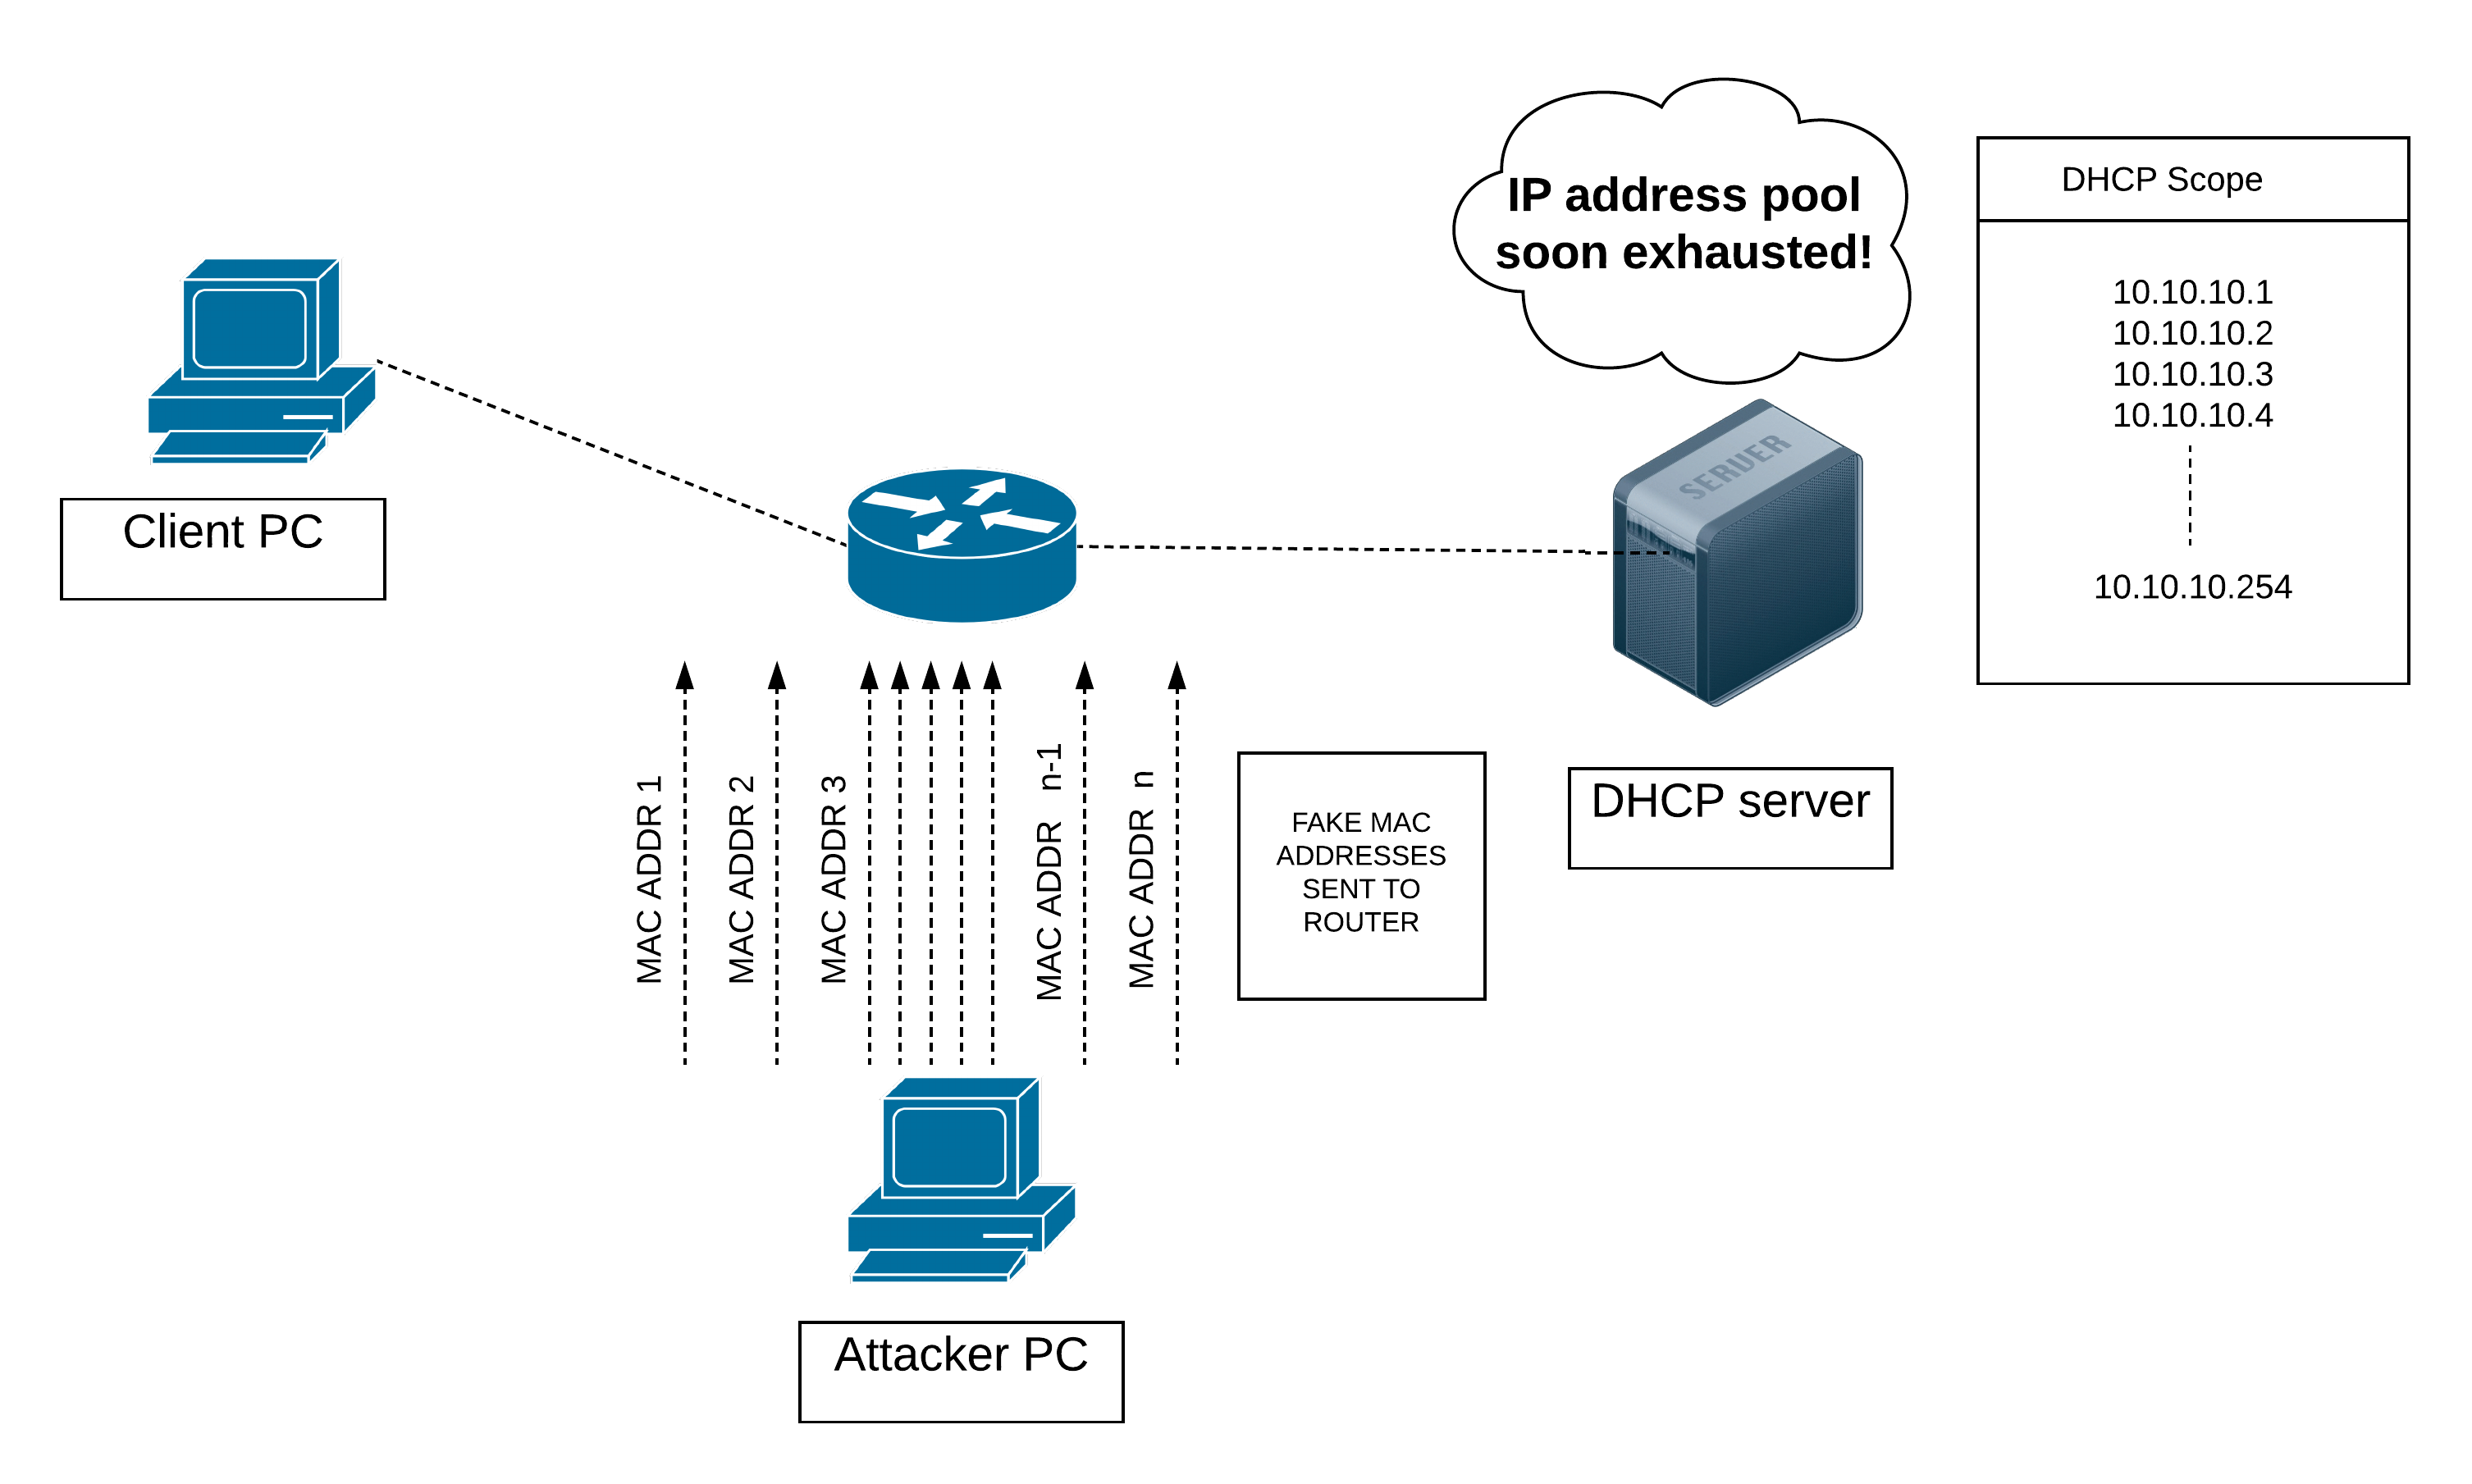
\includegraphics[width=12 cm,height=7 cm]{images/DHCP_STARVATION.png};
		\caption{DHCP starvation}
	\end{figure}

\end{sloppypar}

\section{Attacking strategies and Attack timing diagram}
\subsection{\texttt{\underline{Attacking strategies: Overview} }}

\begin{itemize}
	\item Attacker enables a rouge DHCP server on a network
	
	\item Attacker carries out DHCP starvation attack and depletes the IP address pool of the legal DHCP server.
	
	\item When the client broadcasts a DHCP DISCOVER message, the legal DHCP server cannot send an OFFER because it has no available IP address
	
	\item The fake DHCP server sends out DHCP OFFER acting as the original server
	
	\item Client carries out normal DHCP REQUEST and DHCP ACK operation with the fake server, without having any clue that it is an attacker.
	
\end{itemize}

\subsection{\texttt{\underline{Attacking strategies: Detailed process} }}


\begin{enumerate}
	\item The attacker constructs a DHCP packet with its own MAC address and the DHCP server's IP address and sends the packet to the DHCP client.
	
	\item After receiving the packet, the DHCP client learns the middleman's MAC address. As a result, all the packets sent from the DHCP client to the server pass through the middleman.
	
	\item Alternatively, the middleman constructs a DHCP packet with its own MAC address and the DHCP client's IP address and sends the packet to the DHCP server.
	
	\item After receiving the packet, the DHCP server learns the middleman's MAC address and thinks of it as the client. 
	
	
\end{enumerate}

\textbf{Thus, the DHCP server considers that all packets are sent to or from the DHCP client, and the DHCP client considers that all packets are sent to or from the DHCP server. Packets, however, have been processed on the middleman.}

\begin{figure}[h]
	\centering
	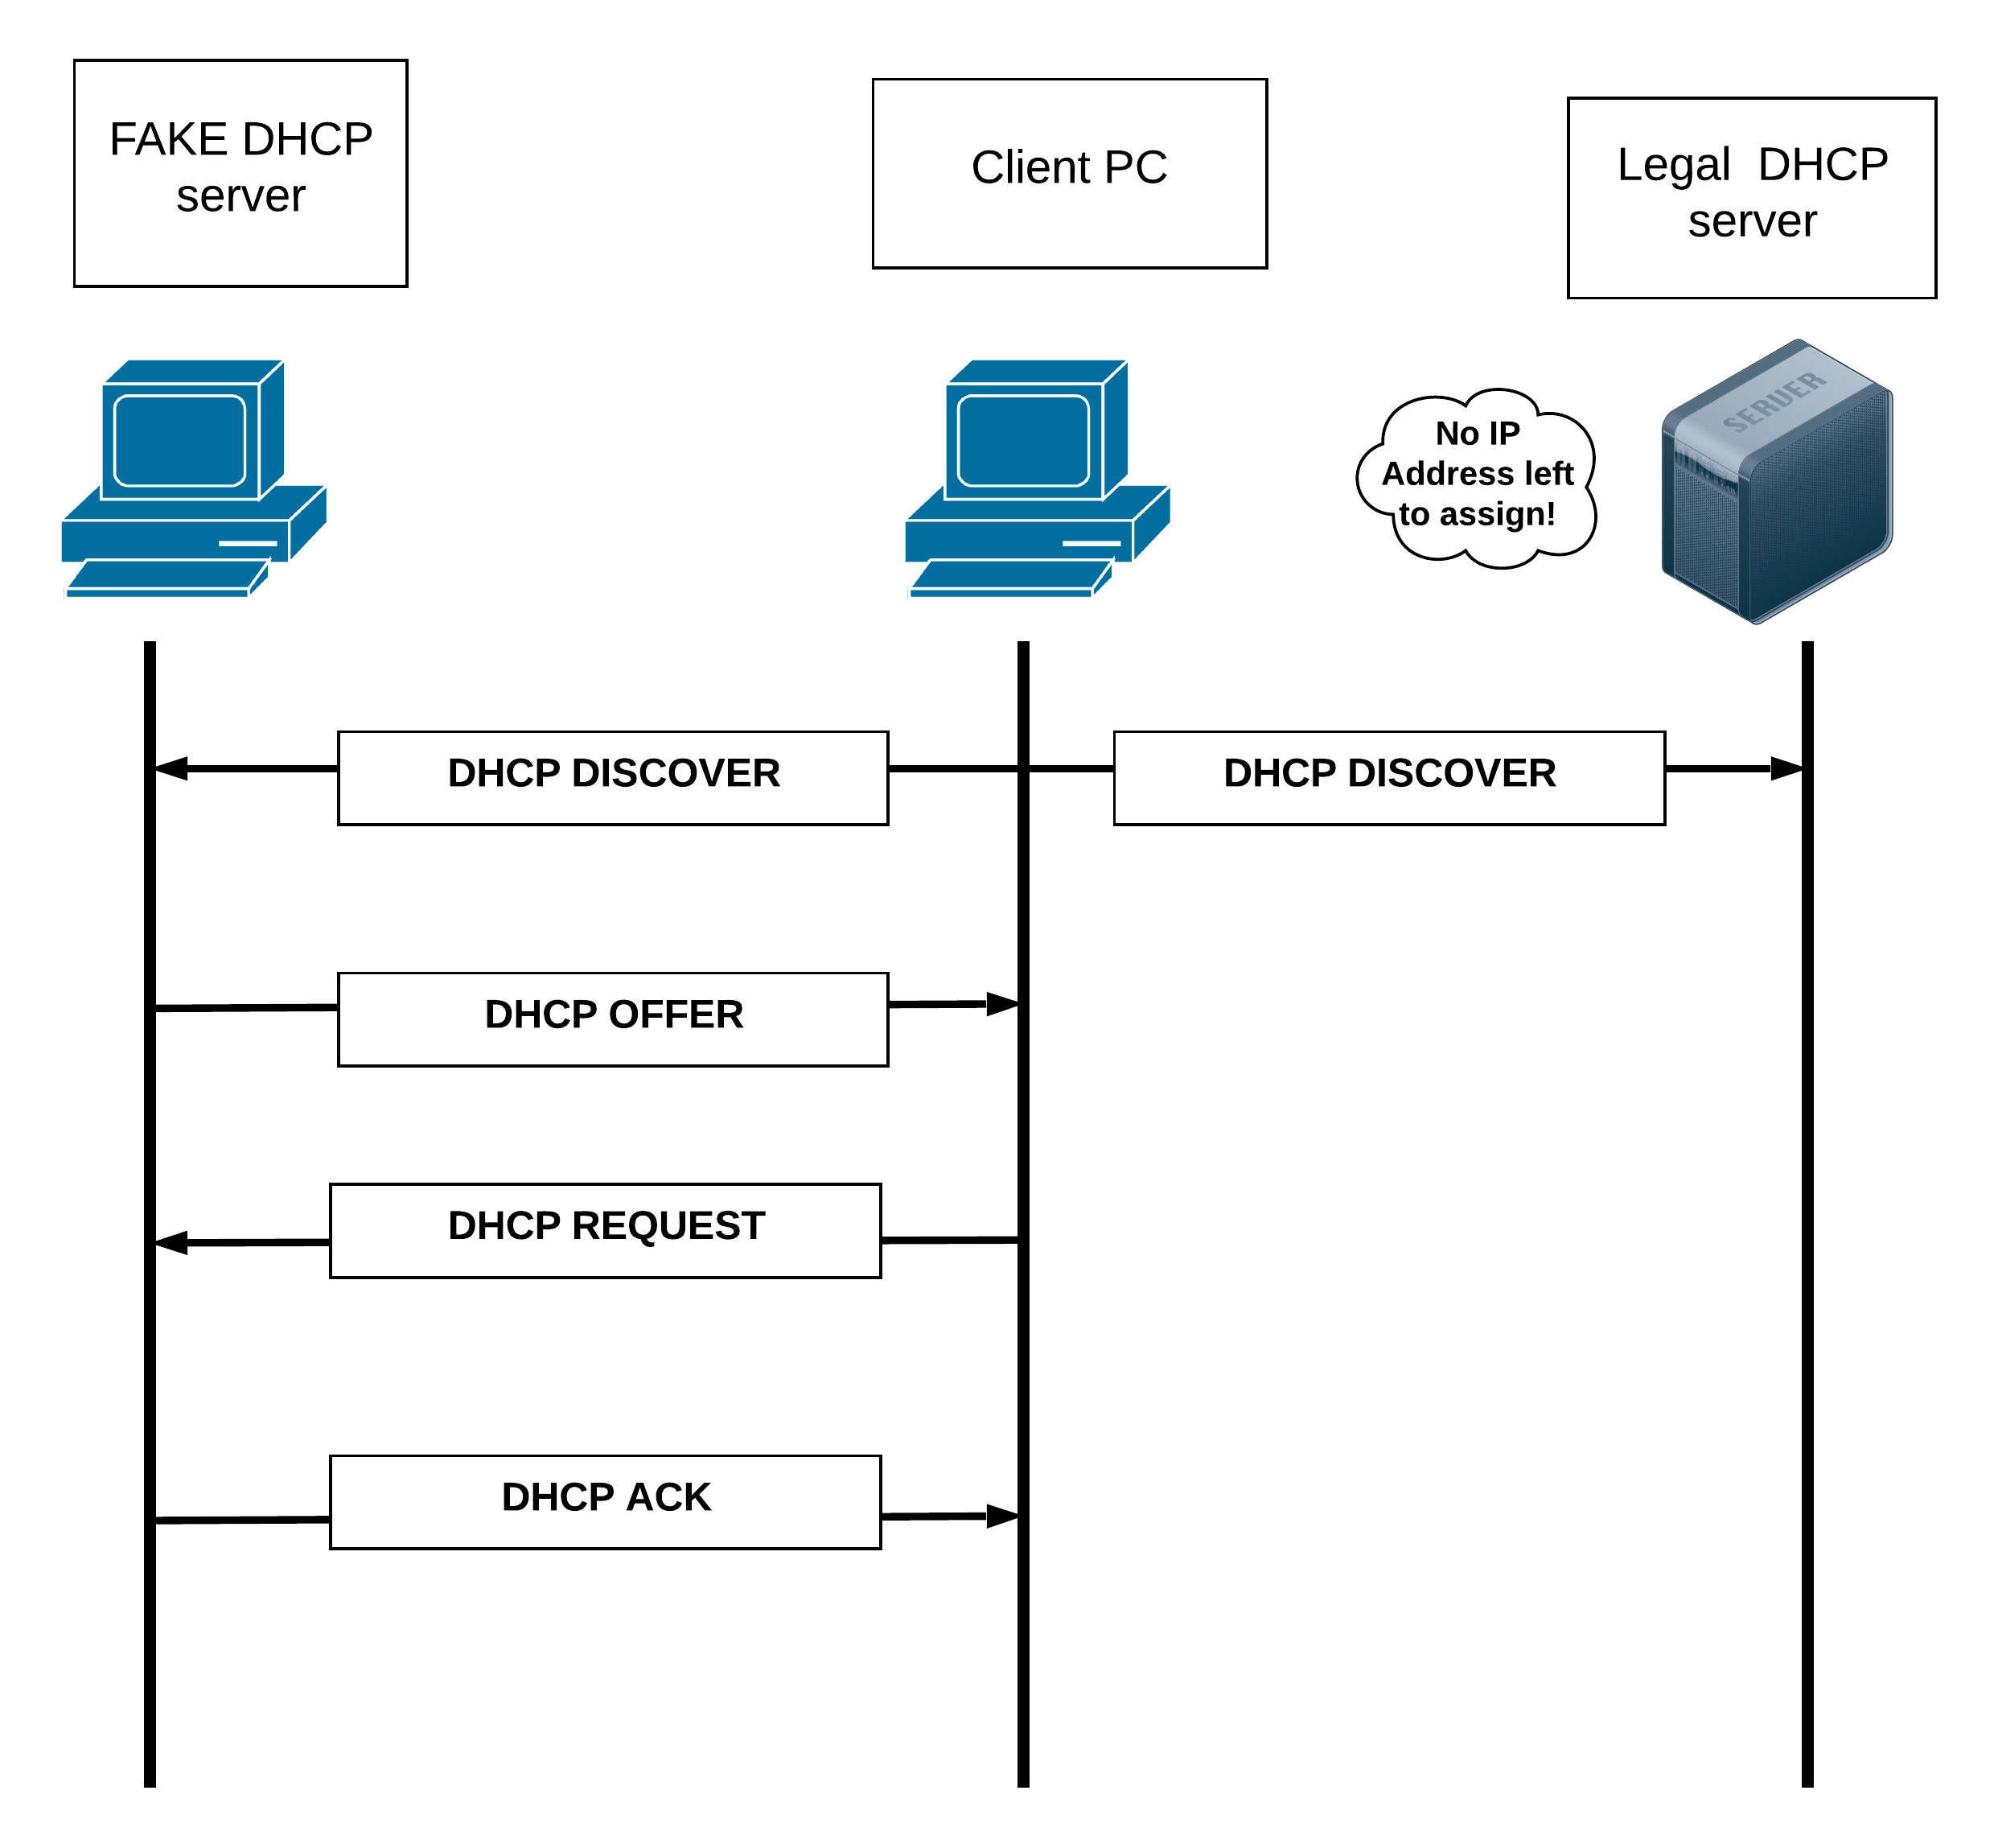
\includegraphics[width=15 cm,height=13 cm]{images/attack_timing.png};
	\caption{Attack Timing Diagram}
\end{figure}

\section{Frame details for the attack with modification}

\subsection{DHCP Frame:}
\begin{figure}[h]
	\centering
	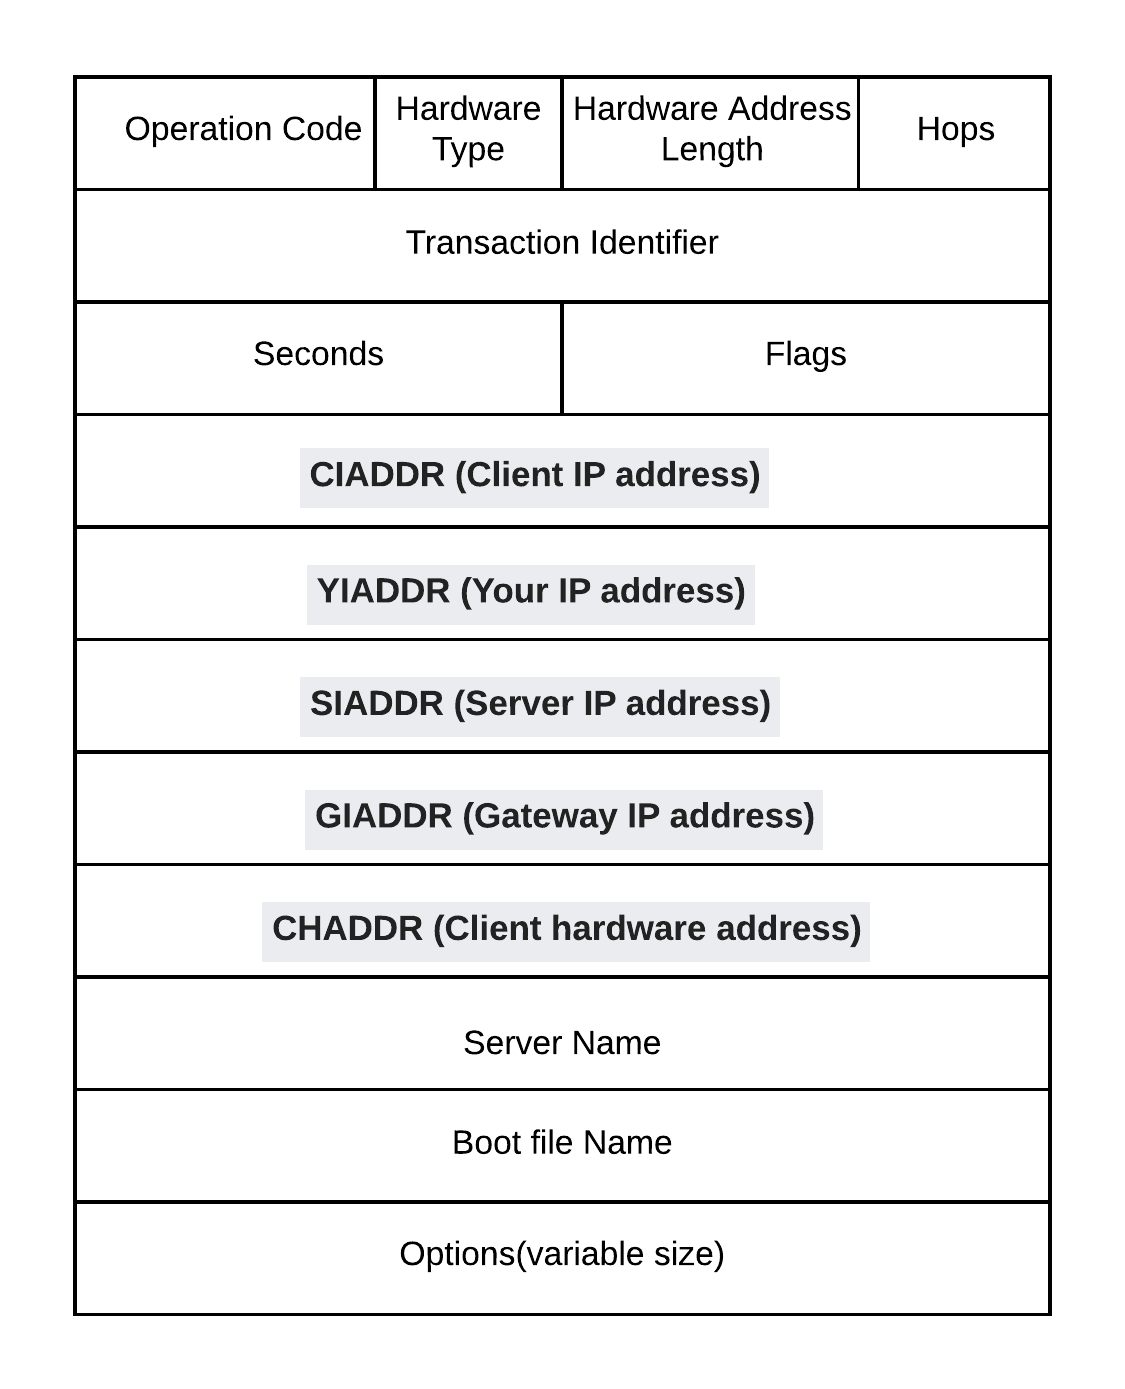
\includegraphics[width=13 cm,height=15 cm]{images/packet_header.png};
	\caption{Example Frame}
\end{figure}

\newpage

\subsection{DHCP message fields}
%
\begin{figure}[!h]
	\centering
	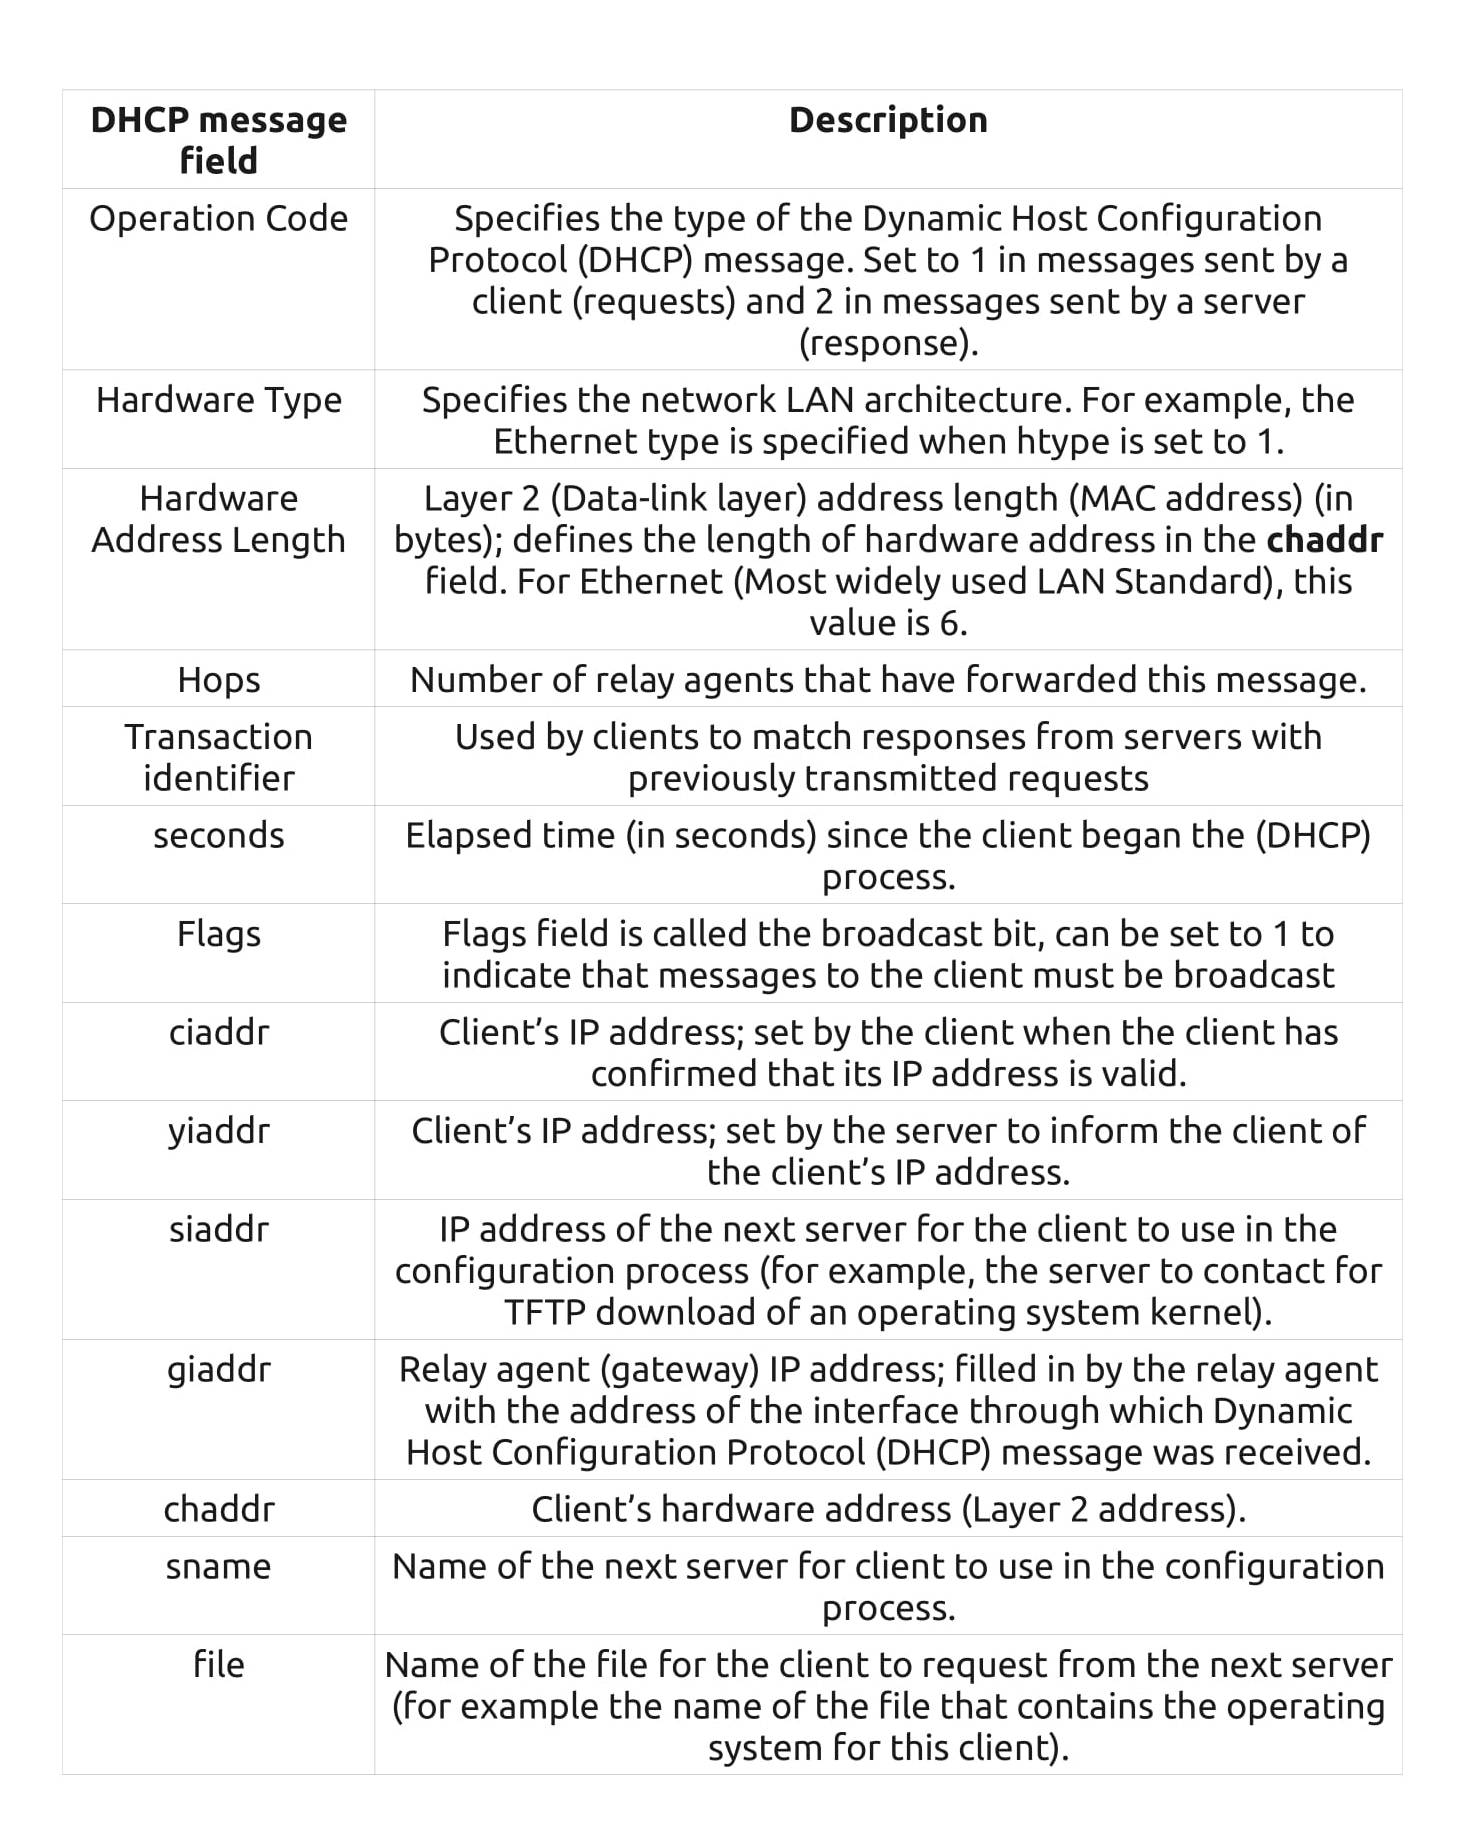
\includegraphics[width=.80\textwidth]{images/msg_fields.jpg};
	\caption{DHCP message fields}
\end{figure}
%

\newpage
\subsection{Example exchange of frames}
%
\begin{figure}[!h]
	\centering
	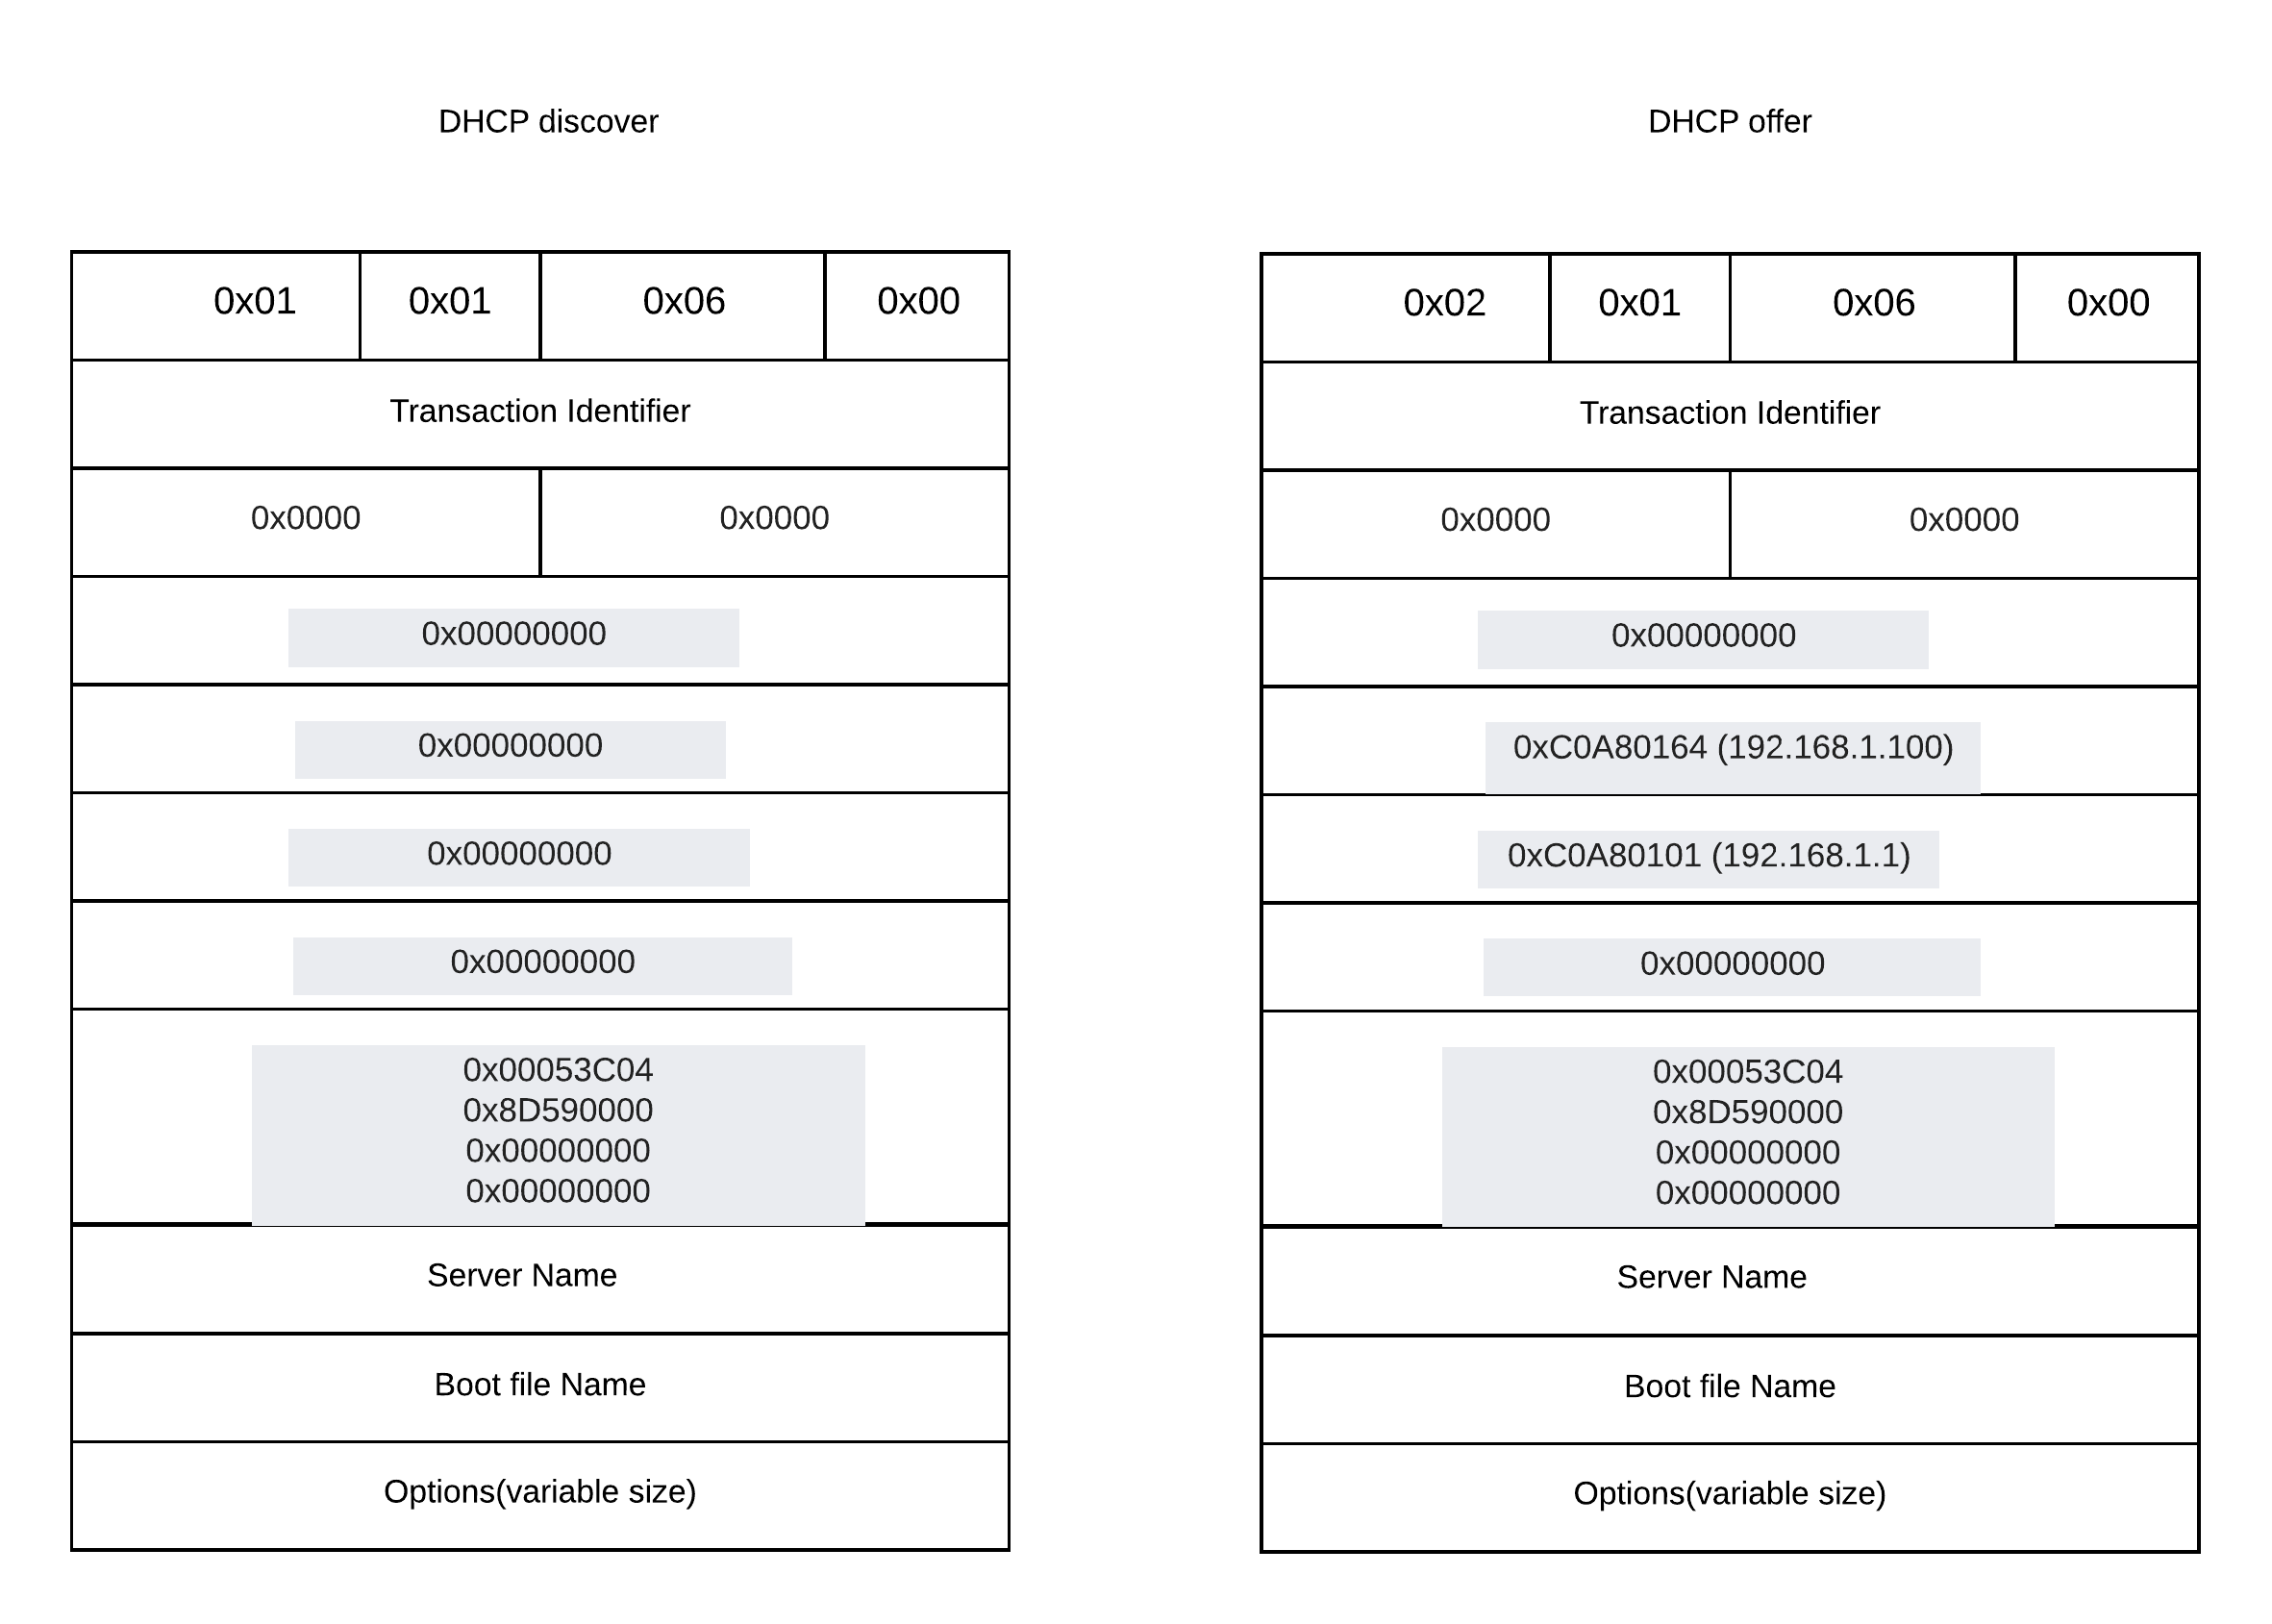
\includegraphics[width=.70\textwidth]{images/packet.png};
	
	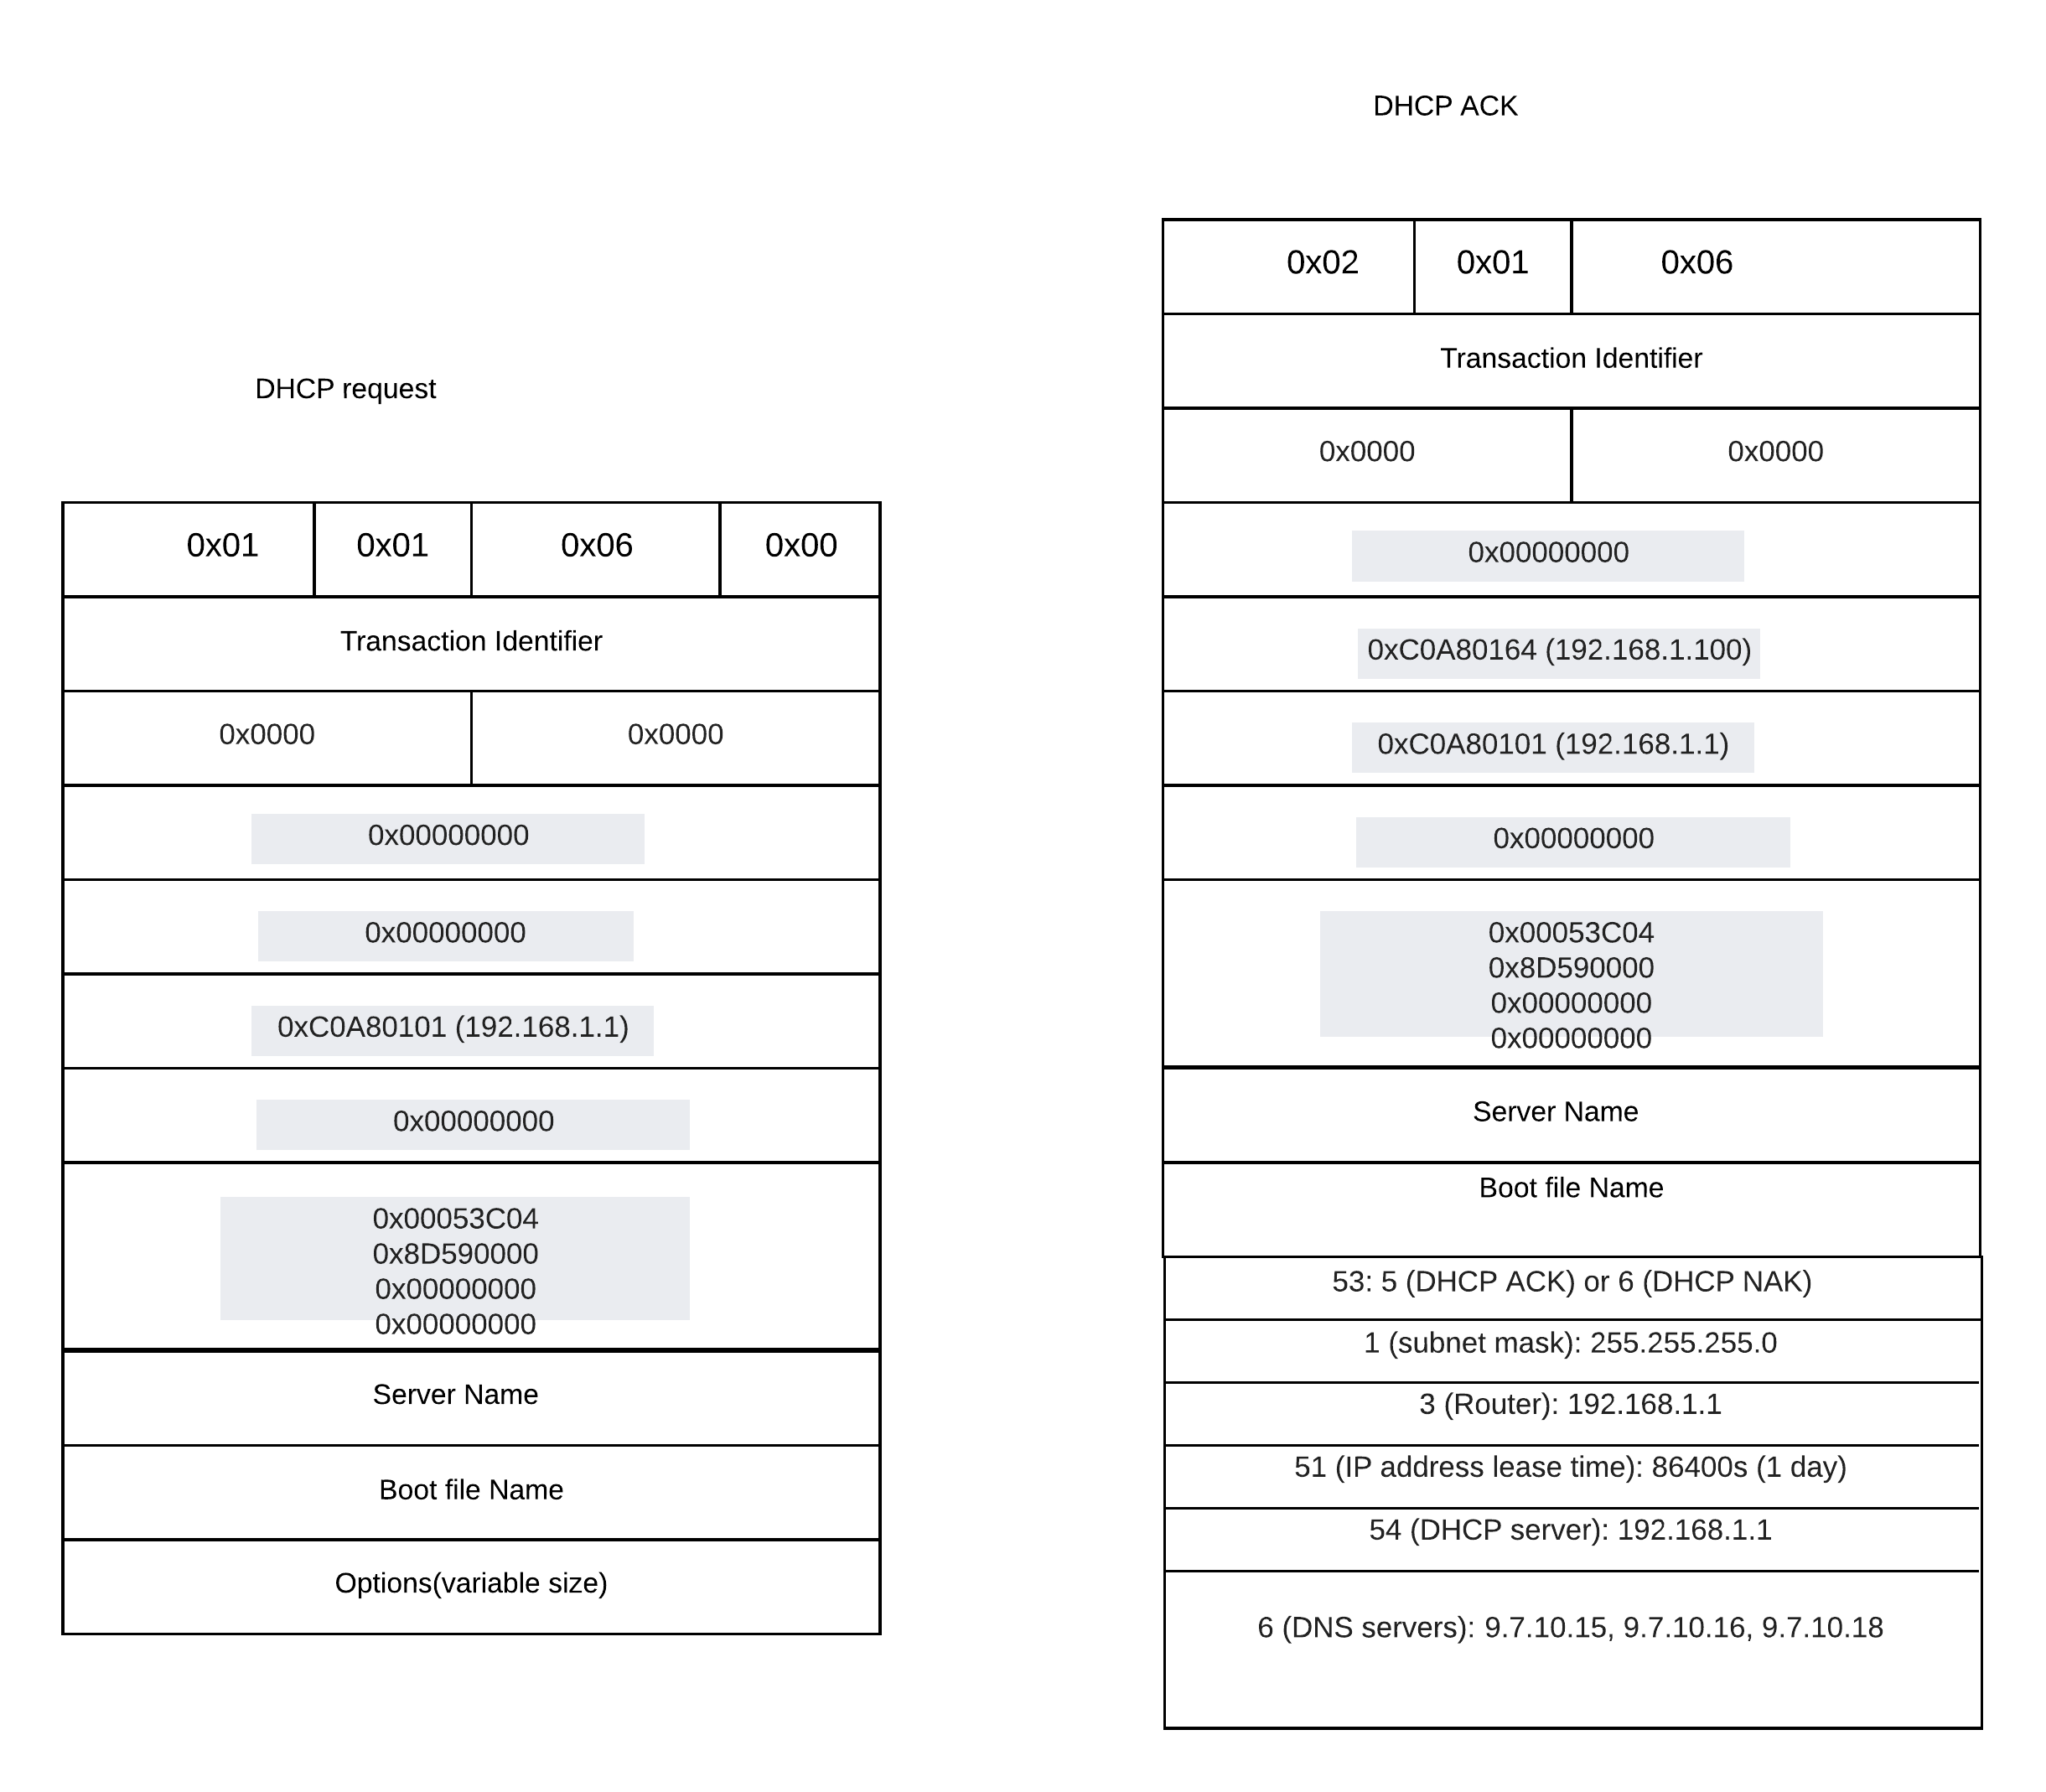
\includegraphics[width=.70\textwidth]{images/packet2.png};
	\caption{Example exchange of frames. Here 0xC0A80101 (192.168.1.1) is the real DHCP IP address which the fake server is using, meanwhile the real server cannot do anything since its IP pool is empty}
\end{figure}
%


\newpage
\section{System Requirements}

\begin{enumerate}
	\item  Install Python following this	\href{http://ubuntuhandbook.org/index.php/2017/07/install-python-3-6-1-in-ubuntu-16-04-lts/}{link}
	
	\item Install Scapy using this \href{https://zoomadmin.com/HowToInstall/UbuntuPackage/scapy}{link}
	
	\item If ubuntu is not booted in your machine, follow this \href{https://itsfoss.com/install-ubuntu-dual-boot-mode-windows/}{link}
	
\end{enumerate}


\newpage
\section{Software/tools/library requirements}

\begin{itemize}
	\item \textbf{Programming language - Python}
	
	
	Python is an interpreted, high-level, general-purpose programming language. Created by Guido van Rossum and first released in 1991, Python's design philosophy emphasizes code readability with its notable use of significant whitespace. 
	
	
	\item \textbf{Library - Scapy (2.3.3)}
	
	Scapy is a packet manipulation tool for computer networks, originally written in Python by Philippe Biondi. It can forge or decode packets, send them on the wire, capture them, and match requests and replies. It can also handle tasks like scanning, tracerouting, probing, unit tests, attacks, and network discovery.	
	
	\item \textbf{Machine used - Ubuntu 18.04}
	
	\item \textbf{Testing tool - Wireshark}
	
	Wireshark is a free and open-source packet analyzer. It is used for network troubleshooting, analysis, software and communications protocol development, and education. 
	
	
\end{itemize}

\section{Setup steps}

Make sure python and scapy is installed, also install wireshark for seeing a detailed info of the packets

\begin{itemize}
	\item run DHCPstarve.py
	\item run DHCPSpoof.py
	\item run dns\_sniff.py
\end{itemize}

Note: If the client or mobile device is already connected to the network this won't work since the router already has a saved IP for your device. ALWAYS PERFORM FORGET NETWORK BEFORE RUNNING




\newpage
\section{Implementation}
\begin{sloppypar}
The implementation is done using scapy which is a packet manipulation tool, written in python. A linux desktop was used as the attacking environment. The router of the wifi network to which the victim and attacker will connect is the good DHCP server. Any device that tries to connect to the wifi network can be labelled as a victim.


\end{sloppypar}

\subsection{Before the attack : }

\begin{figure}[h]
    \centering
    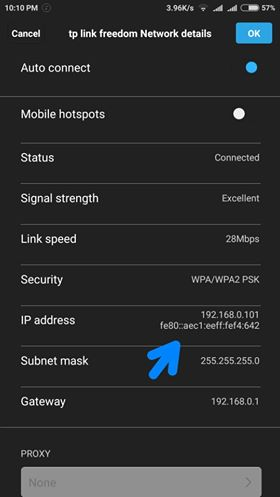
\includegraphics[width=7 cm,height=10 cm]{images/normal_conn.png};
    \caption{Before the attack the client has an ip from a specific pool range}
    \end{figure}


\newpage
\subsection{Steps of the attack}
\subsubsection{Carrying out DHCP Starvation}
\begin{itemize}
     \item Attacker enables a rouge DHCP server on a network.
     
    In this implementation my laptop is acting as the rouge DHCP server.
    
    \item Attacker carries out DHCP starvation attack and depletes the IP address pool of the legal DHCP server.
    
    This is done by running DHCPstarve.py from the attacker PC.
    
    \lstinputlisting[language = Python]{DHCPstarve.py}

    Command Line : 
    \lstinputlisting[language = Python]{cmd1.py}

    \begin{figure}[h]
    \centering
    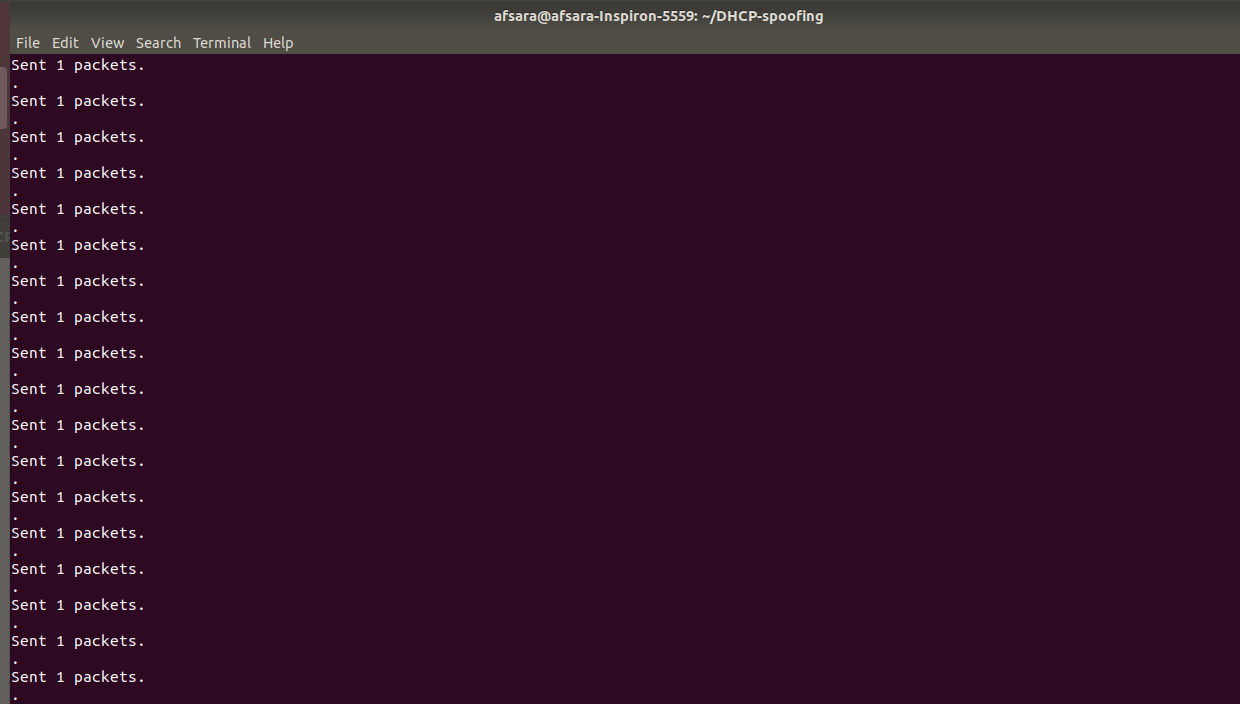
\includegraphics[width=10 cm,height=7 cm]{images/starveConsole.png};
    \caption{Console after running the DHCP starvation attack}
    \end{figure}

     %% image of obtaingin ip oita
    \begin{figure}[h]
    \centering
    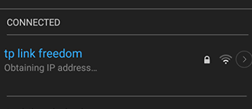
\includegraphics[width=9 cm,height=3 cm]{images/failed_conn.png};
    \caption{Failed Connection}
    \end{figure}
    
    
    \item When the client (\textbf{in this case my Xiaomi mobile device}) tries to connect to the wifi router it fails because the legal DHCP server cannot send an OFFER as it has no available IP address.
    
   
\end{itemize}
    
    

\subsubsection{Carrying out DHCP Spoofing}

\begin{itemize}
  
    \item Now the attacker runs the DHCPSpoof.py which can send a fake ip to any device trying to connect to the network.
    
    \newpage
    DHCPSpoof.py
    \lstinputlisting[language = Python]{DHCPSpoof.py}

    Command Line : 
    \lstinputlisting[language = Python]{cmd2.py}

    \begin{figure}[h]
    \centering
    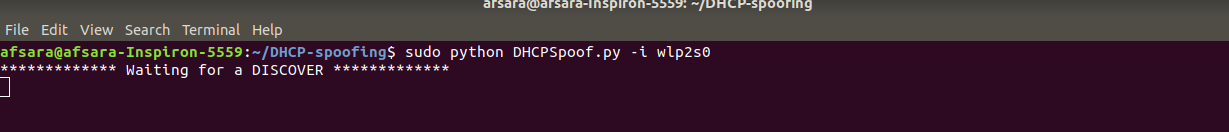
\includegraphics[width=15 cm,height=2 cm]{images/runningDHCPSpoof1.png};
    \caption{My rouge server is waiting for any discover packet to be sent}
    \end{figure}
    
     \item The fake DHCP server sends out DHCP OFFER acting as the original server.
     
     \item Client sends a DHCP request to which the rouge server sends a DHCP ACK.
     
     \item Client thus carries out normal DHCP REQUEST and DHCP ACK operation with the fake server, without having any clue that it is an attacker.
    
    \end{itemize}
    \newpage    
    \section{Demonstrating the attack}

    \begin{figure}[h]
    \centering
    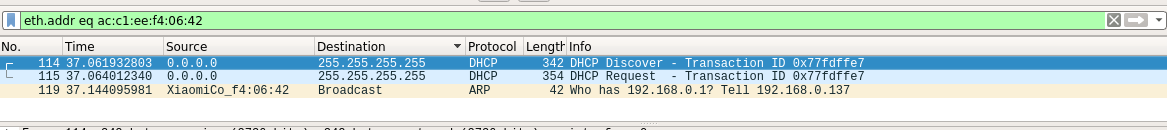
\includegraphics[width=15 cm,height= 3 cm]{images/discover1-1.png};
    \caption{Client sends a broadcast discover packet}
    \end{figure}
    
     \begin{figure}[h]
    \centering
    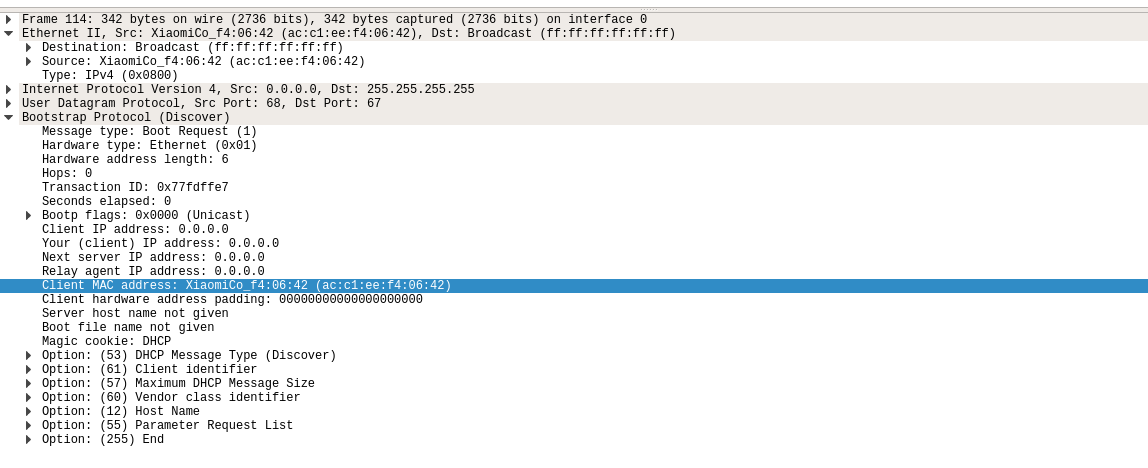
\includegraphics[width=15 cm,height= 9 cm]{images/discover1-2.png};
    \caption{Discover packet description }
    \end{figure}
    
    \newpage
    \begin{figure}[h]
    \centering
    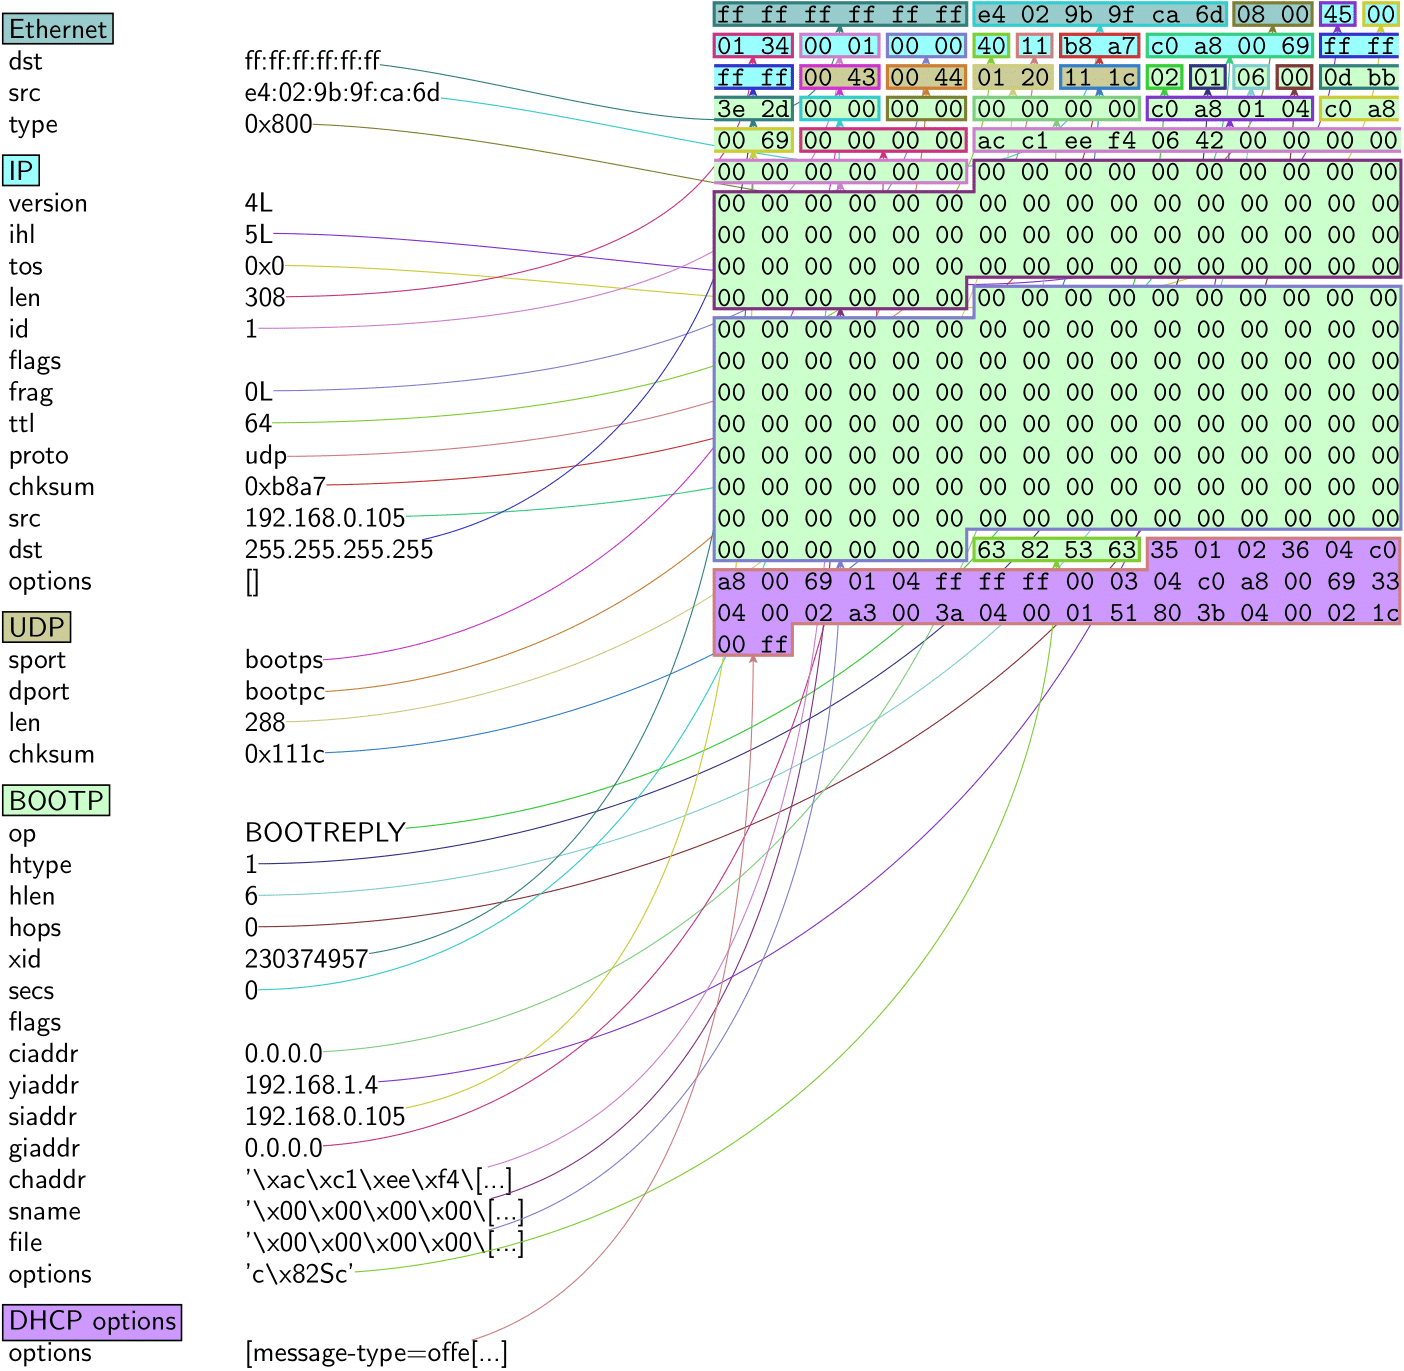
\includegraphics[width=15 cm,height=13 cm]{images/offer-1.png};
    \caption{OFFER packet from rouge server}
    \end{figure}
   
     
    \newpage
    \begin{figure}[h!]
    \centering
    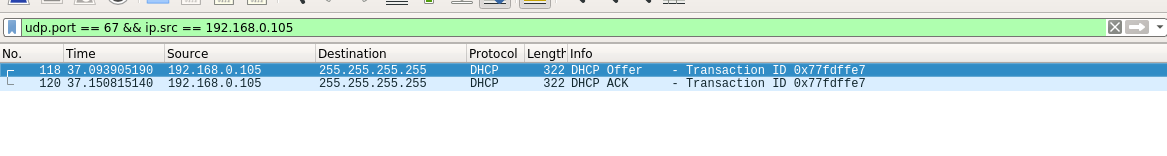
\includegraphics[width=15 cm,height= 3 cm]{images/offer-2-1.png};
    \caption{OFFER packet from rouge server as seen in WireShark}
    \end{figure}
    
    
    \begin{figure}[h!]
    \centering
    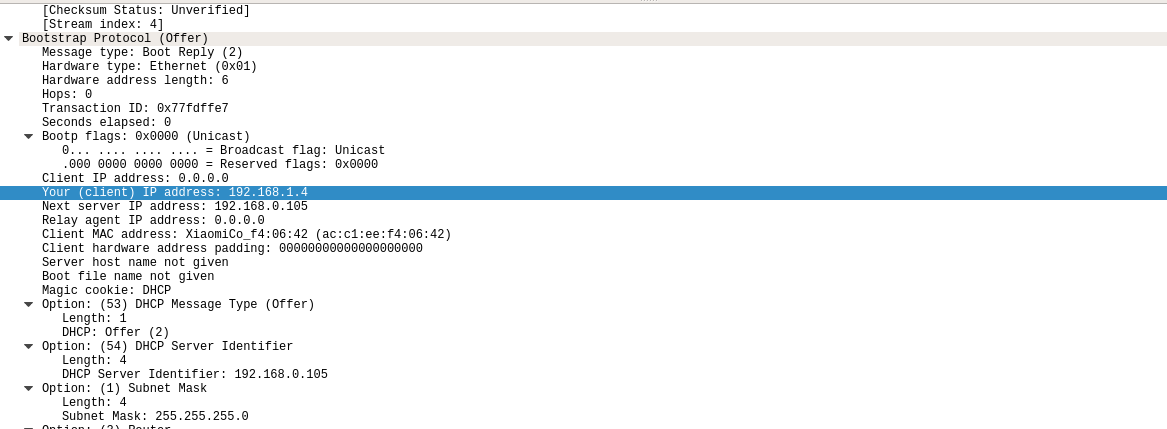
\includegraphics[ width=15 cm,height= 9 cm]{images/offer-2-2.png};
    \caption{ Here client ip offered = 192.168.1.4 and server ip = 192.168.0.105 }
    \end{figure}
    
    
    %%wireshark image jabe of request
    \newpage
    \begin{figure}[h!]
    \centering
    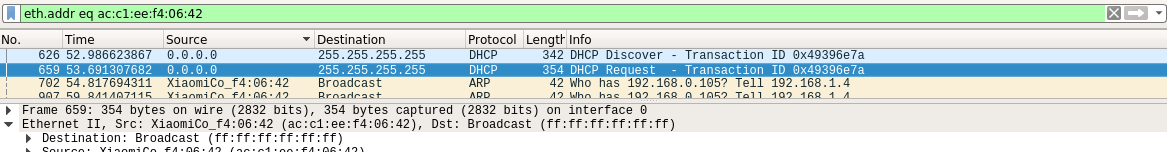
\includegraphics[width=15 cm,height=3 cm]{images/request2-1.png};
    \end{figure}
    
    \begin{figure}[h!]
    \centering
    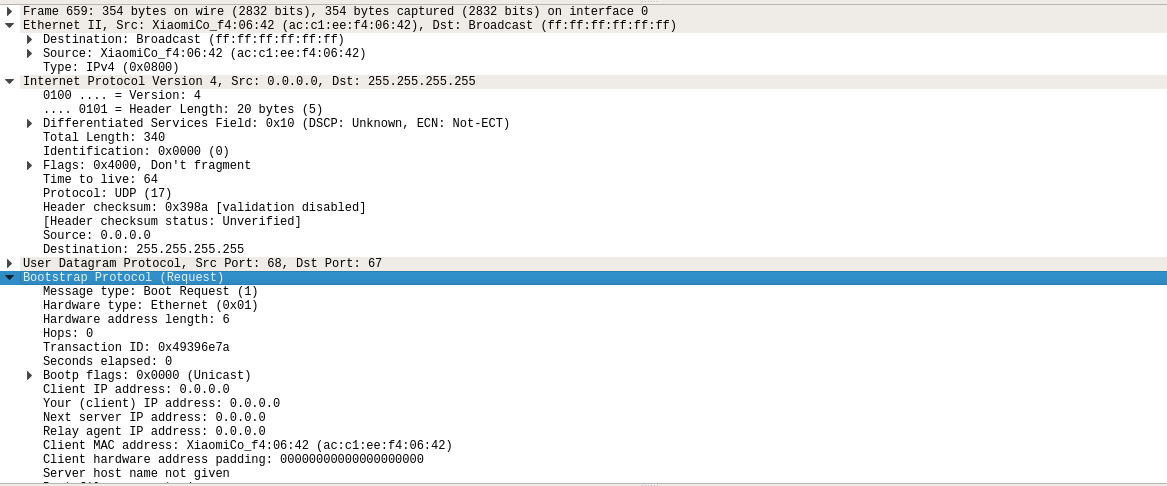
\includegraphics[width=15 cm,height=9 cm]{images/request2-2.png};
    \caption{Request packet from client}
    \end{figure}
    
    
    
    \newpage
    \begin{figure}[h]
    \centering
    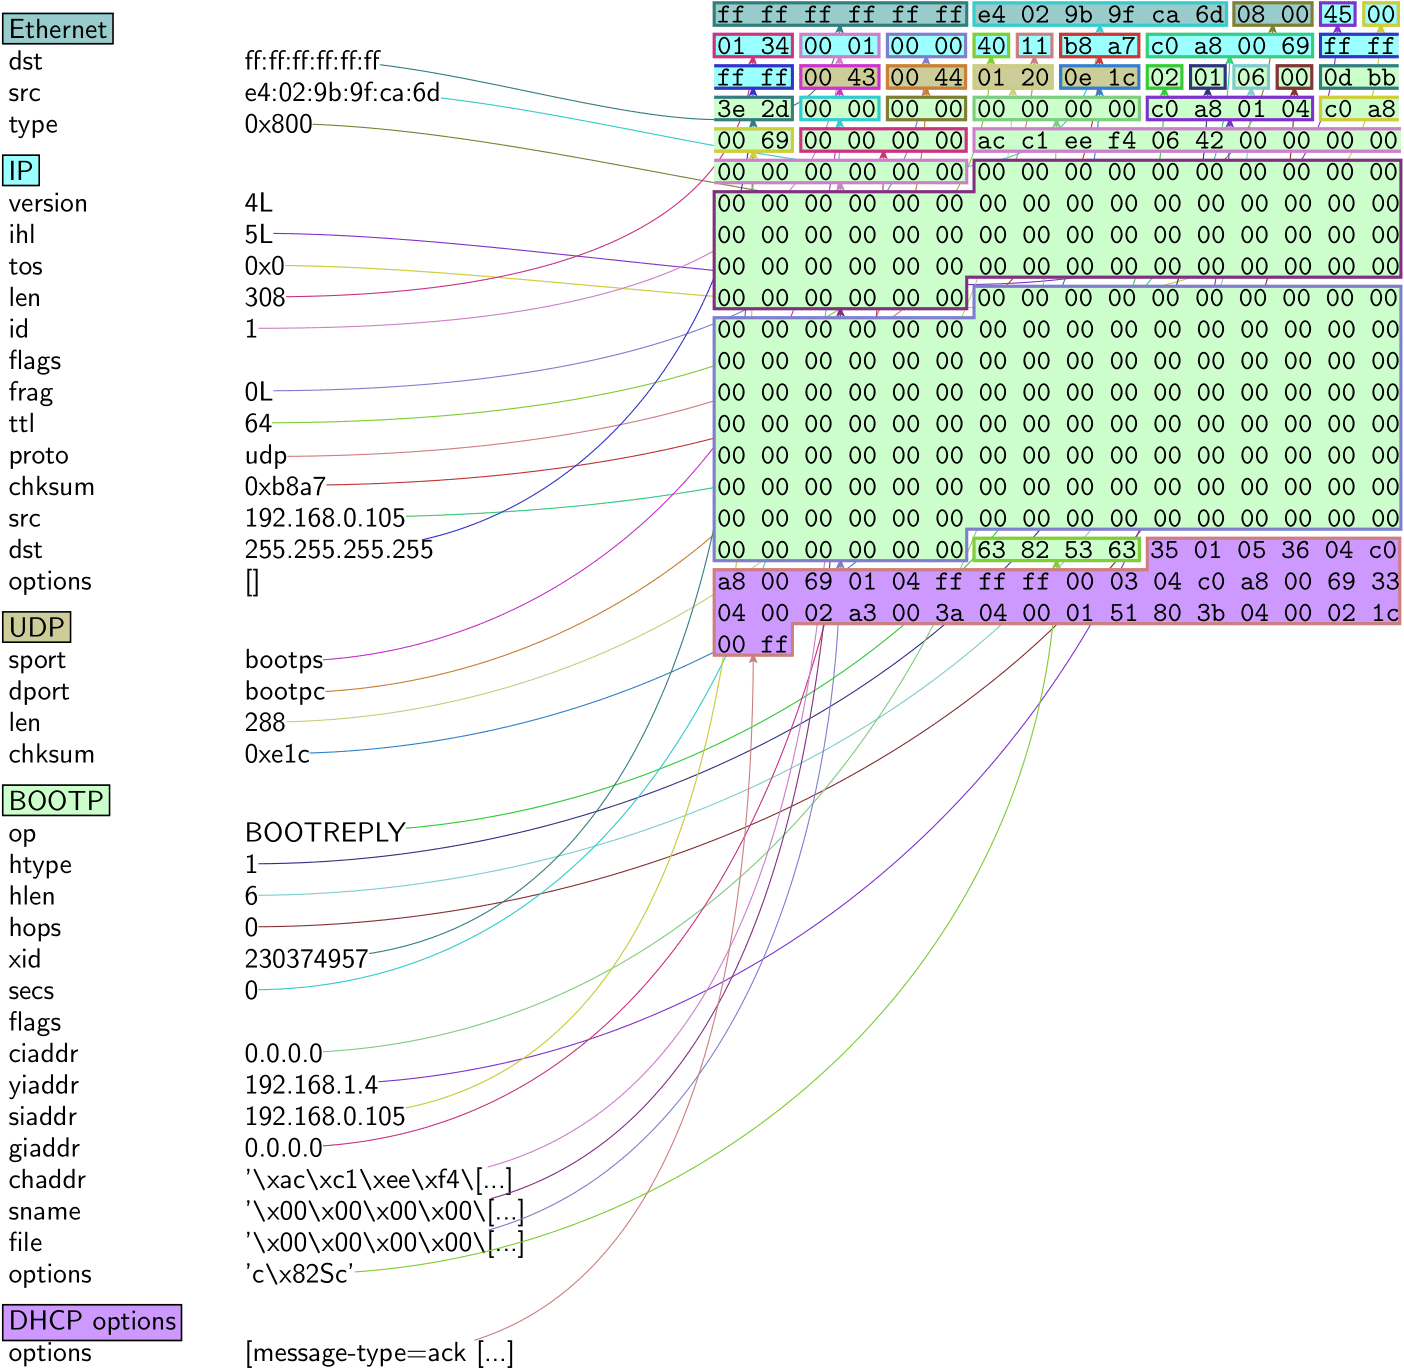
\includegraphics[width=12 cm,height=13 cm]{images/ack-1.png};
    \caption{ACK packet from rouge server}
    \end{figure}
       
       
    \newpage   
    \begin{figure}[h]
    \centering
    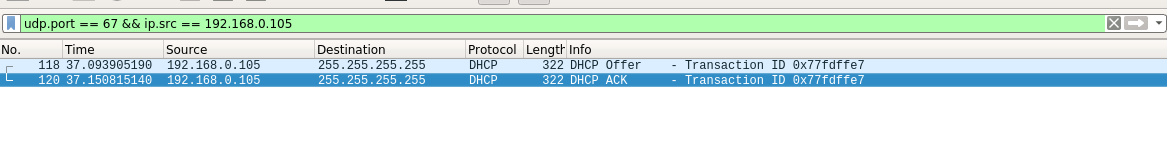
\includegraphics[width=15 cm,height=3 cm]{images/ack-2-1.png};
    
    \end{figure}
    
    
    \begin{figure}[h]
    \centering
    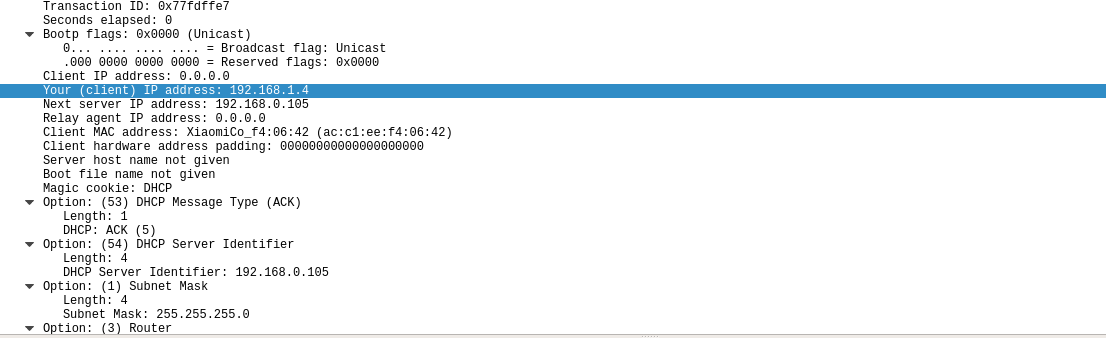
\includegraphics[width=15 cm,height=7 cm]{images/ack-2-2.png};
    \caption{ACK packet from rouge server as seen in WireShark}
    \end{figure}
    
        
    
    
    
    %fake ip dekhaba of client
    \newpage
    \begin{figure}[h]
    \centering
    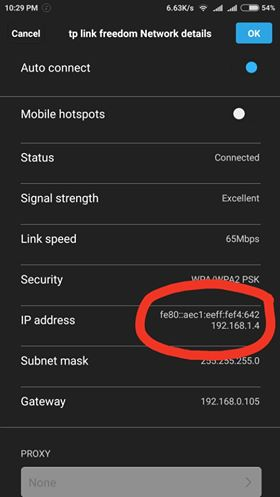
\includegraphics[width=7 cm,height=10 cm]{images/spoofed_conn.png};
    \caption{Client now has a fake IP from the attacker}
    \end{figure}
    

\subsection{Performing DNS sniff}

 \lstinputlisting[language = Python]{dns_sniff.py}

\newpage
    \begin{figure}[h]
    \centering
    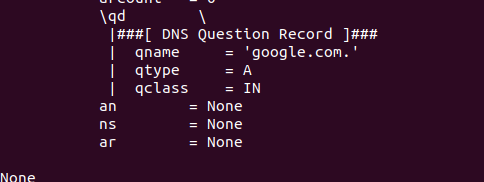
\includegraphics[width=9 cm,height=3 cm]{images/sniff-1.png};
    \caption{Sniffed query}
    \end{figure}
\end{sloppypar}


% \newpage
% \newpage
 \section{Success and Limitations}
\begin{sloppypar}

The attack was successful in the sense that the victim could be successfully assigned a fake IP, when it tried to connect to the network, as was intended.

But needless to say only assigning a fake ip to a victim is of no use if we cannot resolve their DNS queries. Connecting the victim through the gateway of the attacker would have enabled the attacker to see all the DNS requests and redirect those requests as the attacker wishes.

But in this implementation, the network connection of the victim turns off since there is no gateway to connect to the outer world. It keep on trying to connect to the outer world with a fake ip. 

Resolving and redirecting the DNS queries of the victim is a man in the middle attack, which doesn't explicitly fall under DHCP spoofing (although the purpose of spoofing is to perform a MITM).

\end{sloppypar}


\section{Countermeasure}

DHCP Snooping is a Layer 2 security switch feature which blocks unauthorized (rogue) DHCP servers from distributing IP addresses to DHCP clients. 

It is important to note that DHCP SNOOPING is an access layer protection service – it does not belong in the core network.

The way DHCP Snooping works is fairly straight forward. DHCP Snooping categorizes all switch ports into two simple categories:

\begin{enumerate}
    \item Trusted Ports
    \item Untrusted Ports
\end{enumerate}

A Trusted Port, also known as a Trusted Source or Trusted Interface, is a port or source whose DHCP server messages are trusted because it is under the organization’s administrative control. 

An Untrusted Port, also known as an Untrusted Source or Untrusted Interface, is a port from which DHCP server messages are not trusted. An example on an untrusted port is one where hosts or PCs connect to from which DHCP OFFER, DHCP ACK or DHCPNAK messages should never be seen as these are sent only by DHCP Servers.

When enabling DHCP Snooping the switch will begin to drop specific type of DHCP traffic in order to protect the network from rogue DHCP servers. 

DHCP Snooping will drop DHCP messages DHCPACK, DHCPNAK, DHCPOFFER originating from a DHCP server that is not trusted – that is, connected to an untrusted port.

\subsection{\texttt{\underline{Why the prevention wasn't implemented? }}}

Because the given implementation is done using a wireless router and \textbf{Port security is purely for wired connected }. Each device is connected to the router by means of a switch.

\newpage
\section{Other ways of implementation}

\subsection{\texttt{\underline{Using Mininet and Ettercap} }}
Another approach of demonstrating DHCP spoofing is creating a virtual router and network environment and carrying on the attack there.

Mininet creates a realistic virtual network, running real kernel, switch and application code, on a single machine (VM, cloud or native), in seconds, with a single command.And Ettercap is a free and open source network security tool for man-in-the-middle attacks on LAN. 

Using mininet and ettercap a DHCP spoof attack might have been possible but due to the restriction that we cannot use an in-built tool like ettercap for passing messages, this method was not followed.


\subsection{\texttt{\underline{Alternative of starvation} }}

If we have the router access to a network, its IP pool range can be changed so that the IP's assigned to devices in the MAC address table does not exist anymore. Then the client must have to use the fake IP offered by the attacker, since its previous IP range is no more configurable by the router

\newpage
\section{Resources}
\begin{enumerate}
	\item DHCP protocol : \href{http://www.networksorcery.com/enp/protocol/dhcp.htm}{1} \href{https://en.wikipedia.org/wiki/Dynamic_Host_Configuration_Protocol}{2} \href{ https://learningnetwork.cisco.com/docs/DOC-24355}{3}
	
		
	\item DHCP message format : \href{http://www.omnisecu.com/tcpip/dhcp-dynamic-host-configuration-protocol-message-format.php}{1} \href{https://www.whitewinterwolf.com/posts/2017/10/30/dhcp-exploitation-guide/}{2}

	\item subnets and IP addresses : \href{https://routersecurity.org/ipaddresses.php#targetText=A\%20common\%20IP\%20address\%20is,is\%20visible\%20on\%20the\%20Internet.}{1}
	
	
	\item DHCP Starvation : \href{https://www.youtube.com/watch?v=7RJ1Pn4Fl9Q&t=106s}{1} \href{https://github.com/shreyasdamle/DHCP-Starvation-/blob/master/dhcp_starvation.py}{2} \href{https://github.com/avaiyang/dhcp-starvation-attack/blob/master/dhcp\_starve.py}{3} 
	
	\item DHCP Spoof : \href{https://github.com/byt3bl33d3r/DHCPShock/blob/master/dhcpshock.py}{1} \href{https://support.huawei.com/enterprise/en/doc/EDOC1100058937/40d3ec1/man-in-the-middle-attack-ip-mac-spoofing-attack-and-dhcp-exhaustion-attack}{2}
	
	 
	
	\item Scapy cheatsheet : \href{	https://blogs.sans.org/pen-testing/files/2016/04/ScapyCheatSheet_v0.2.pdf}{1} 
	

	
	\item Scapy documentation : \href{	https://buildmedia.readthedocs.org/media/pdf/scapy/latest/scapy.pdf}{1}
	

	
	\item Python Docs : \href{	https://docs.python.org/2/library/argparse.html}{1}
	

	
	\item Scapy listener in python : \href{	https://jcutrer.com/python/scapy-dhcp-listener
	}{1}
	

	\item Packet sniffer : \href{https://medium.com/@777rip777/packet-sniffer-with-scapy-part-3-a895ce7e9cb}{1}
	
	
	
	\item DHCP snooping : \href{https://orhanergun.net/2017/03/layer-2-security-dhcp-details-dhcp-snooping/}{1}  \href{http://www.firewall.cx/cisco-technical-knowledgebase/cisco-switches/1215-understanding-dhcp-snooping-concepts-and-how-it-works.html}{2} 
	
	\item DHCP spoof using Mininet : \href{https://github.com/floft/dhcp-spoof}{1} 
	
	\item MITM : \href{https://seclists.org/vuln-dev/2002/Sep/99}{1} \href{https://security.stackexchange.com/questions/172687/what-is-the-role-of-arp-poisoning-when-doing-a-dhcp-spoofing-attack?newreg=05b564b9b8374bb7af97e9917fc967bc}{2}
	
	
	
	\item Others \href{	https://stackoverflow.com/questions/44937242/how-to-determine-if-an-ip-packet-is-dhcp-packet
	}{1} \href{	https://stackoverflow.com/questions/50026438/crafting-a-dhcp-offer-packet-in-scapy}{2} \href{https://stackoverflow.com/questions/22720788/dhcp-release-using-scapy}{3} \href{https://stackoverflow.com/questions/57811366/continue-net-connection-of-victim-after-dhcp-spoofing-attack}{text} 
	\href{https://medium.com/@lucideus/dhcp-starvation-attack-with-dhcp-rogue-server-lucideus-research-68b2447de7d0}{text}
	
	\item Preventing DHCP starvation in real world : \href{http://www.revolutionwifi.net/revolutionwifi/2011/03/preventing-dhcp-starvation-attacks.html}{1} \href{https://www.cisco.com/c/en/us/td/docs/switches/lan/catalyst3560/software/release/12-2_44_se/configuration/guide/scg/swdhcp82.html#wp1078853}{2}
	
	
	
\end{enumerate}









\end{document}
